\chapter{Casos de Uso}
\label{Anexo:casos}
En este anexo se presenta a trav�s de im�genes los tres casos de uso comentados en esta memoria.

\lsection{Caso 1}
\label{Anexo:caso1}
Recordemos este caso de uso. El usuario debe abrir el men� desplegable y apagar el sistema. Su finalidad es probar el sistema de interacci�n del sistema.

\begin{figure} [H]
\centering	
	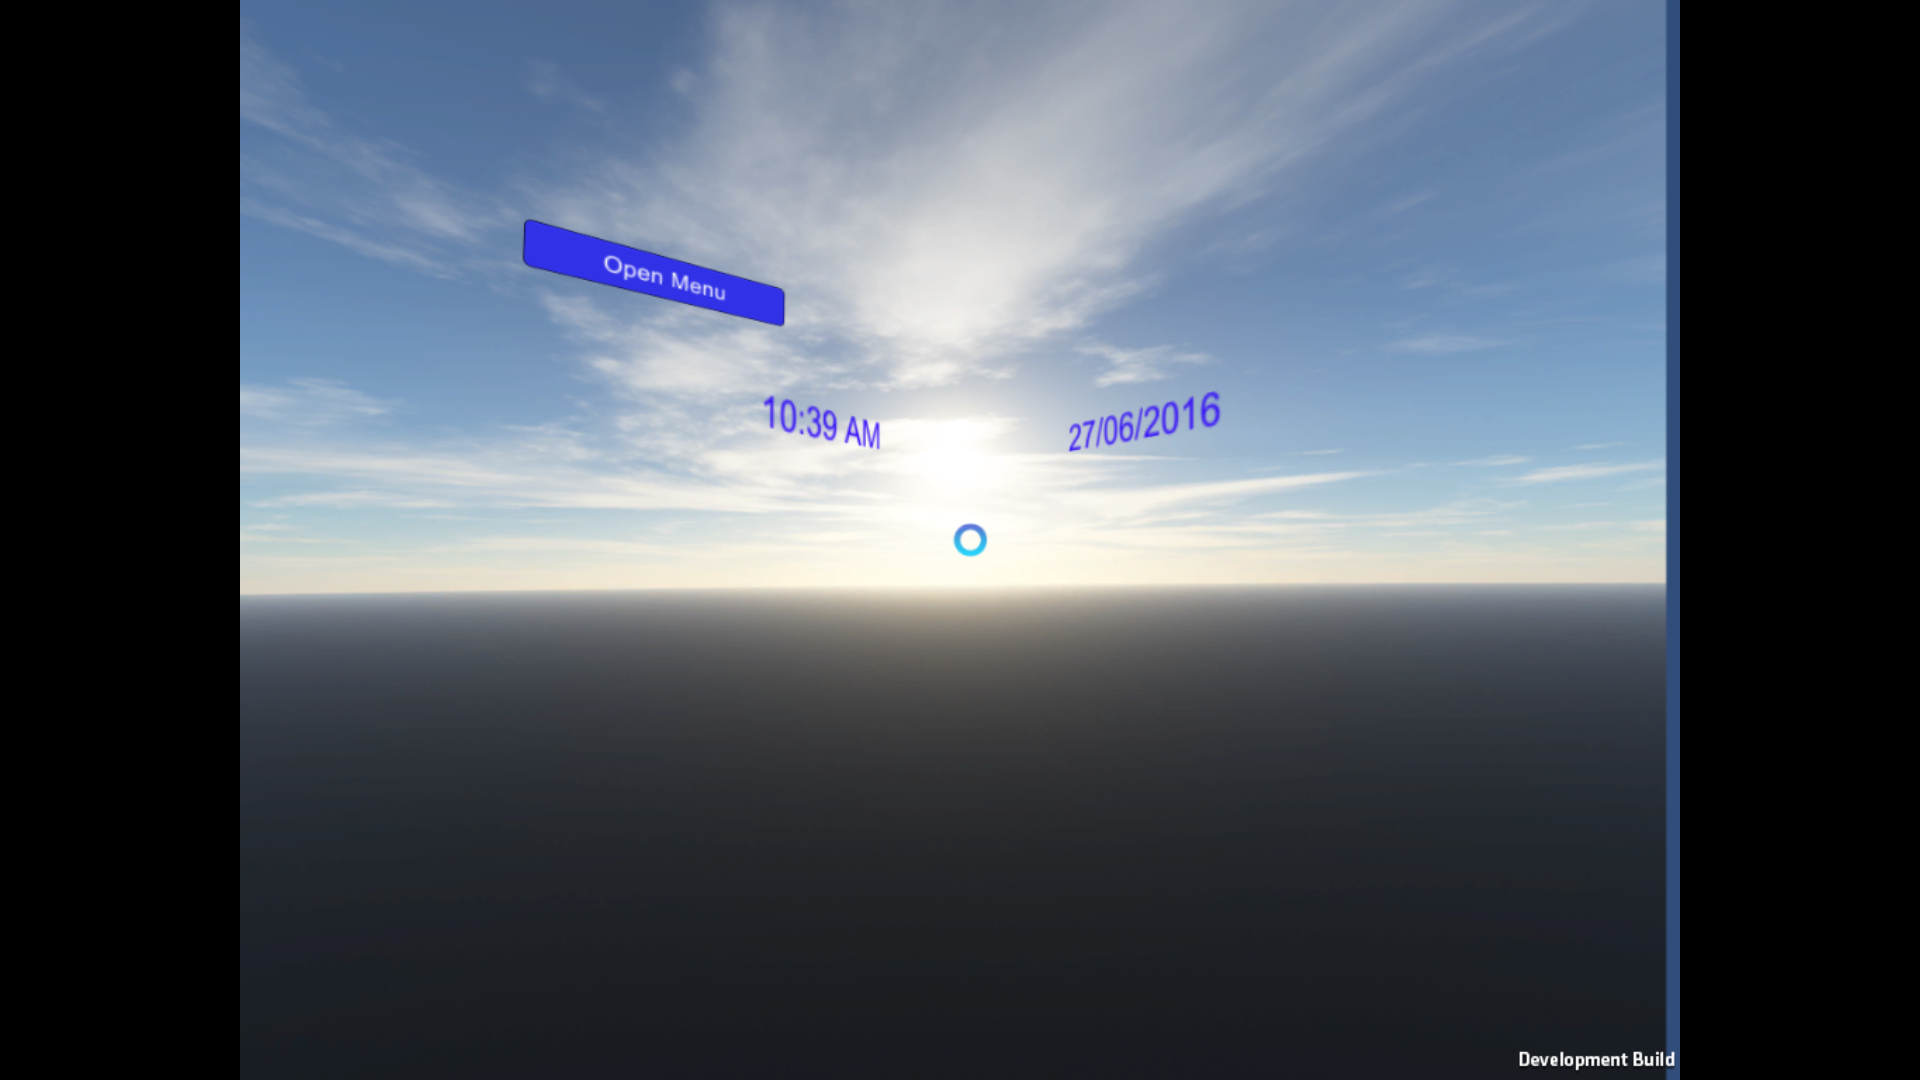
\includegraphics[width=\textwidth]{images/inicio.png} 
  \caption{Pantalla de inicio del sistema.}
  \label{fig:init1}
\end{figure}

\begin{figure} [H]
\centering	
	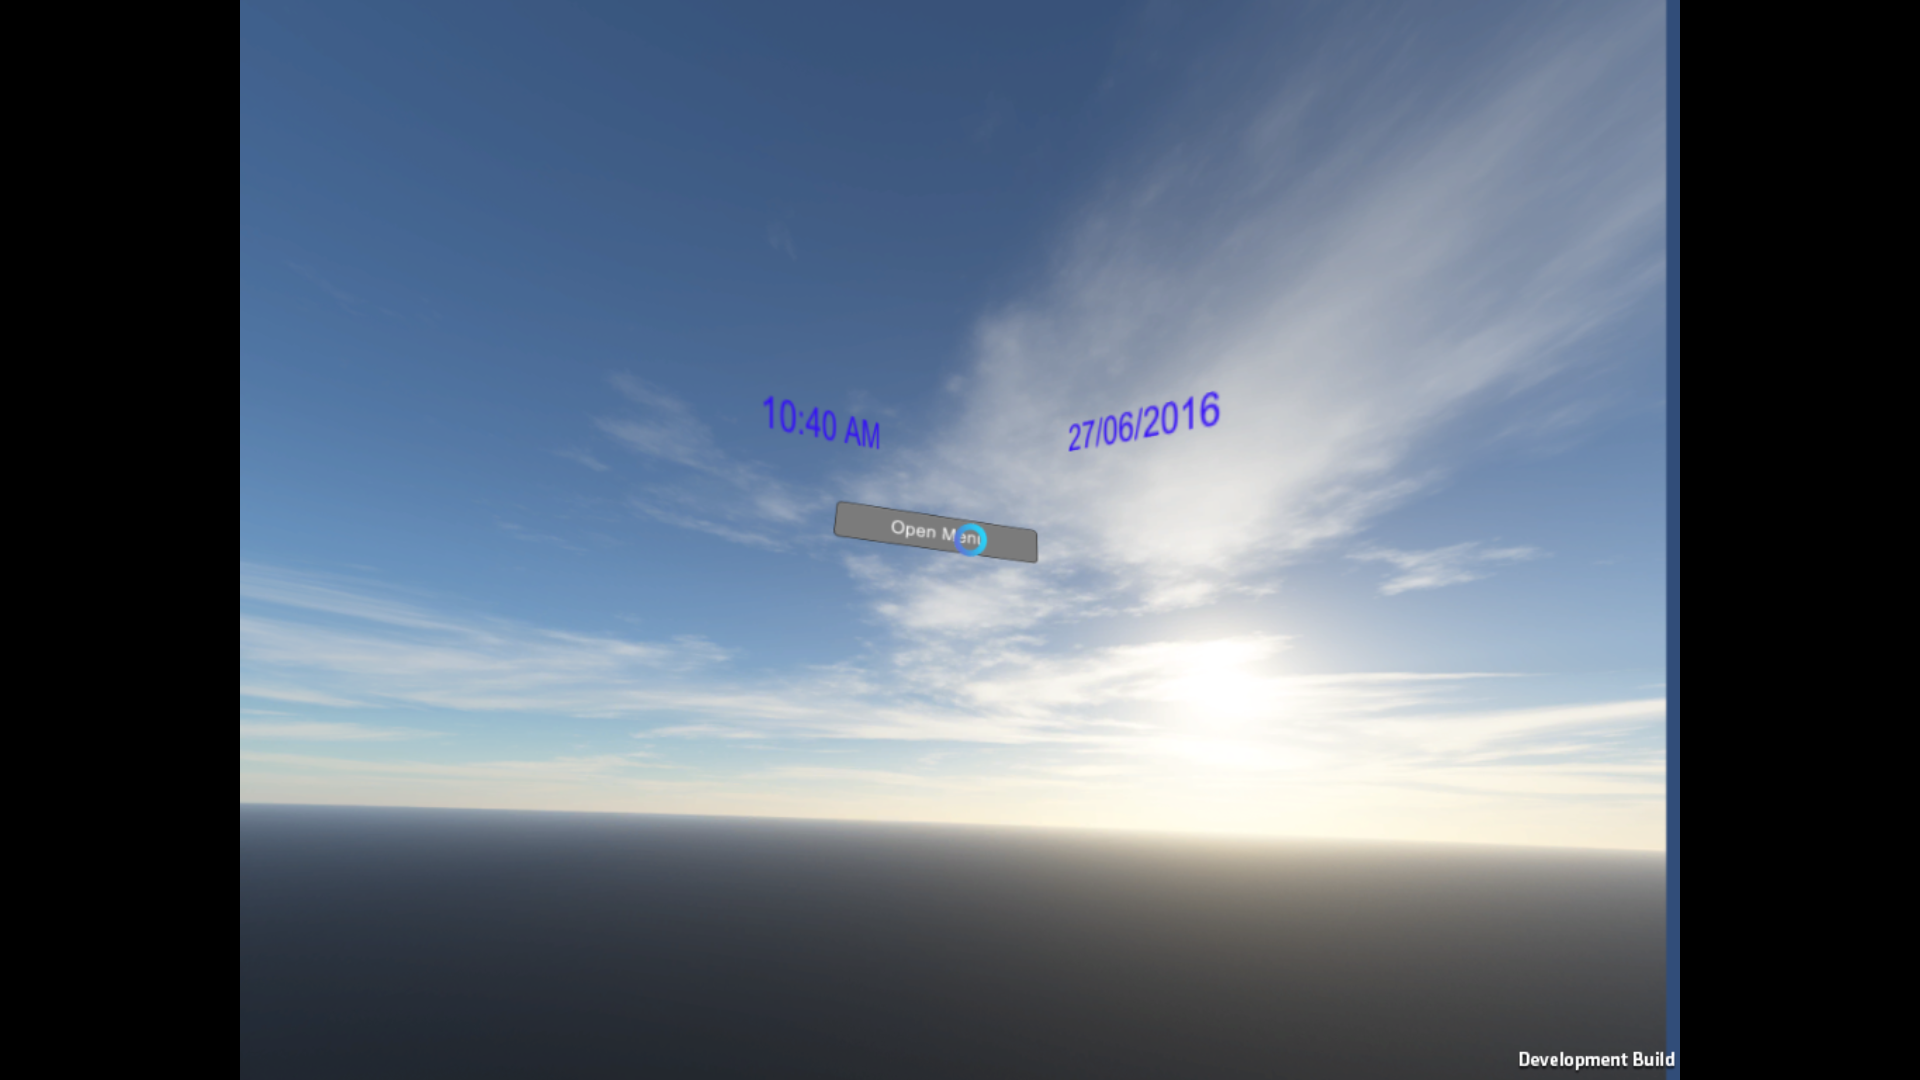
\includegraphics[width=\textwidth]{images/int_menu_open.png} 
  \caption{Usuario seleccionado la opci�n para abrir el men�.}
  \label{fig:openMenu1}
\end{figure}

\begin{figure} [H]
\centering	
	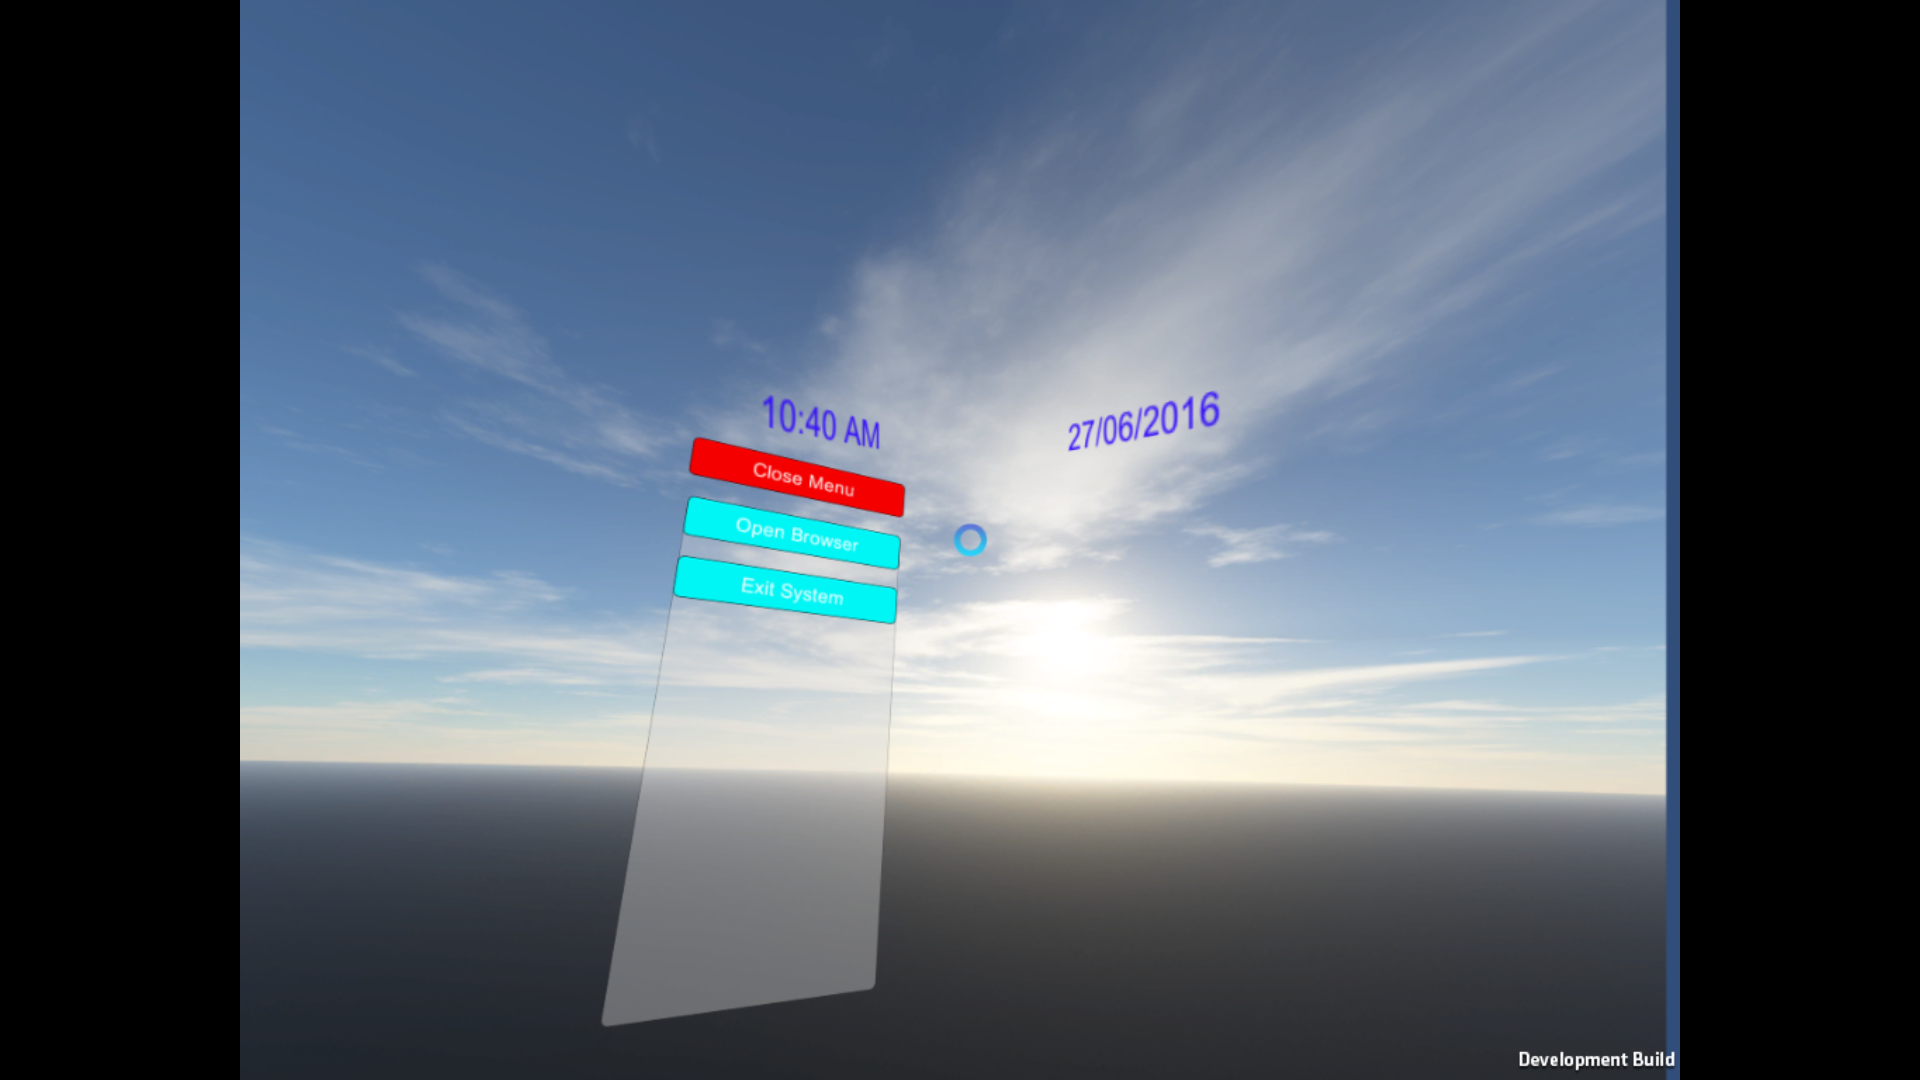
\includegraphics[width=\textwidth]{images/menu_abierto.png} 
  \caption{Men� desplegado.}
  \label{fig:menu1}
\end{figure}

\begin{figure} [H]
\centering	
	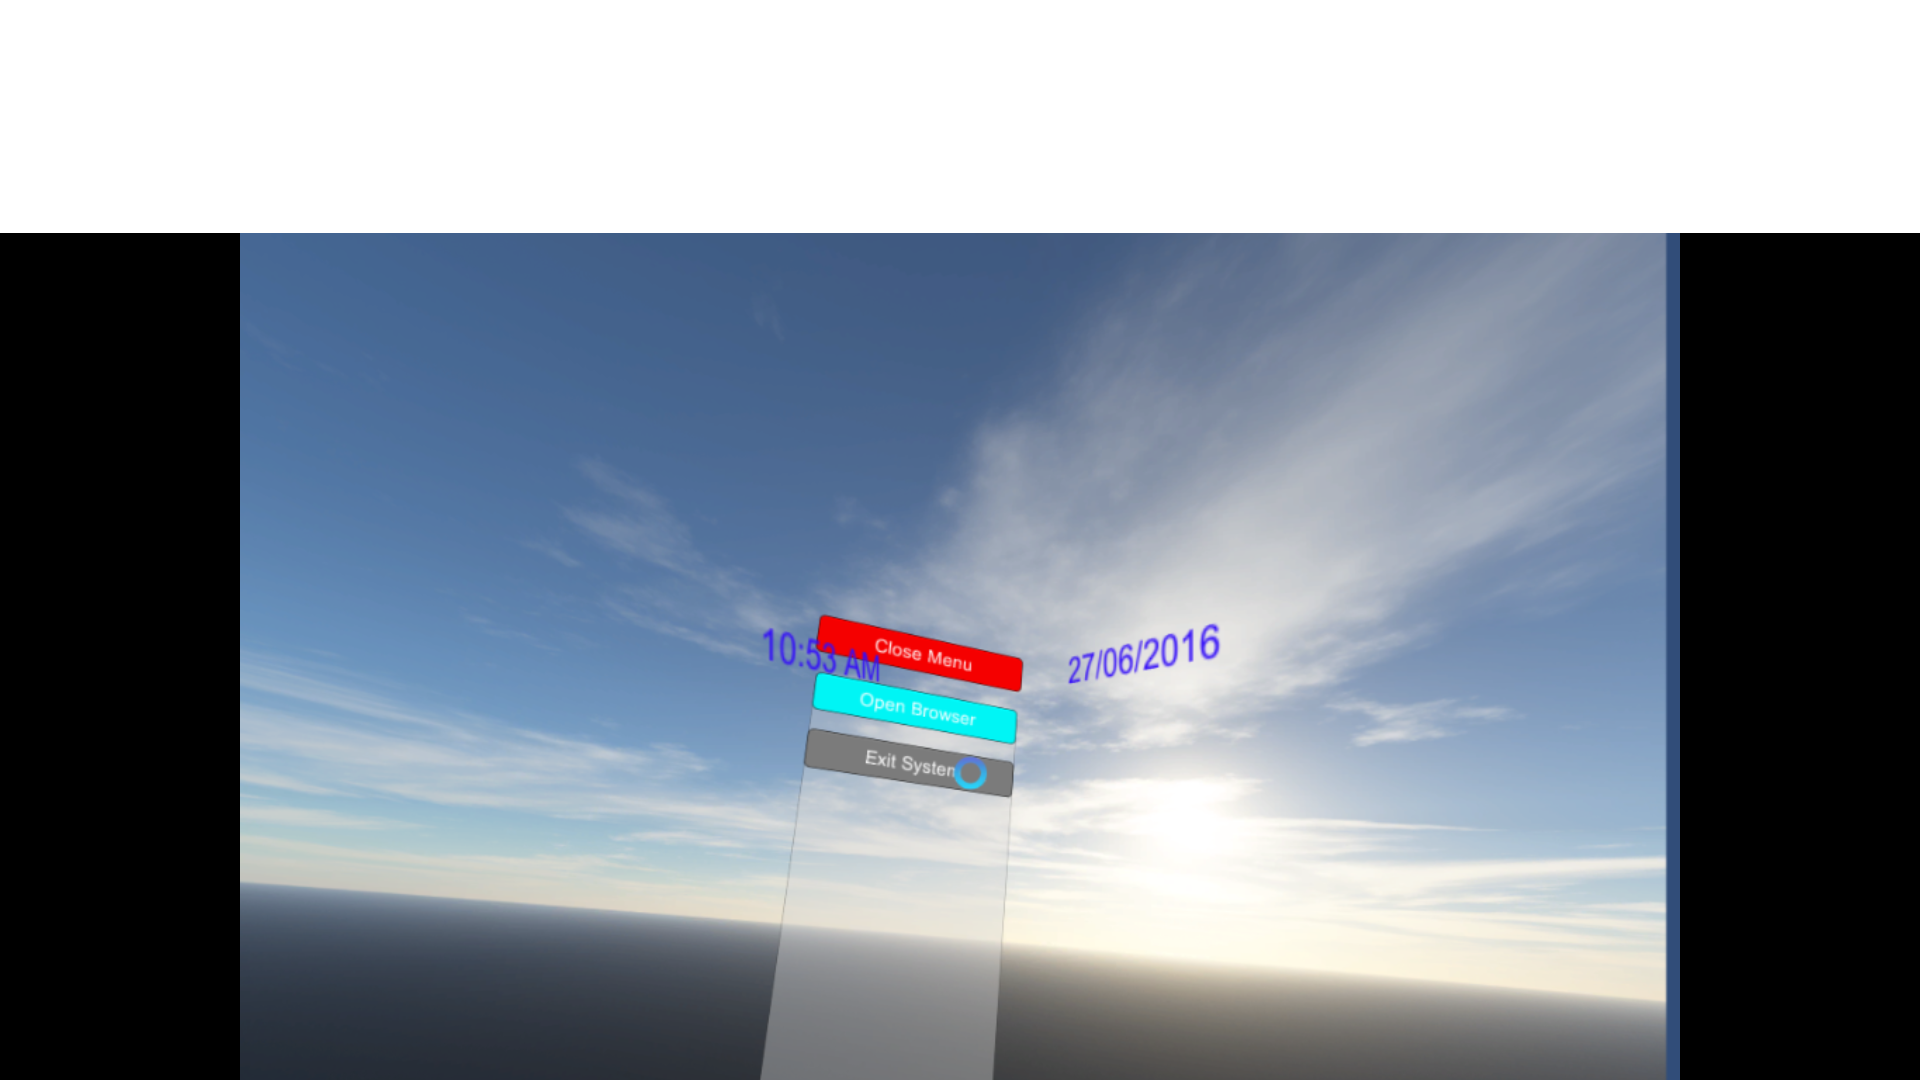
\includegraphics[width=\textwidth]{images/salir_sistema.png} 
  \caption{Usuario seleccionado la opci�n para apagar el sistema.}
  \label{fig:exit1}
\end{figure}

\lsection{Caso 2}
\label{Anexo:caso2}
Recordemos este caso de uso. El usuario debe abrir el men� desplegable y seleccionar la opci�n del navegador. Tras eso debe cerrar dicho navegador y el sistema.

\begin{figure} [H]
\centering	
	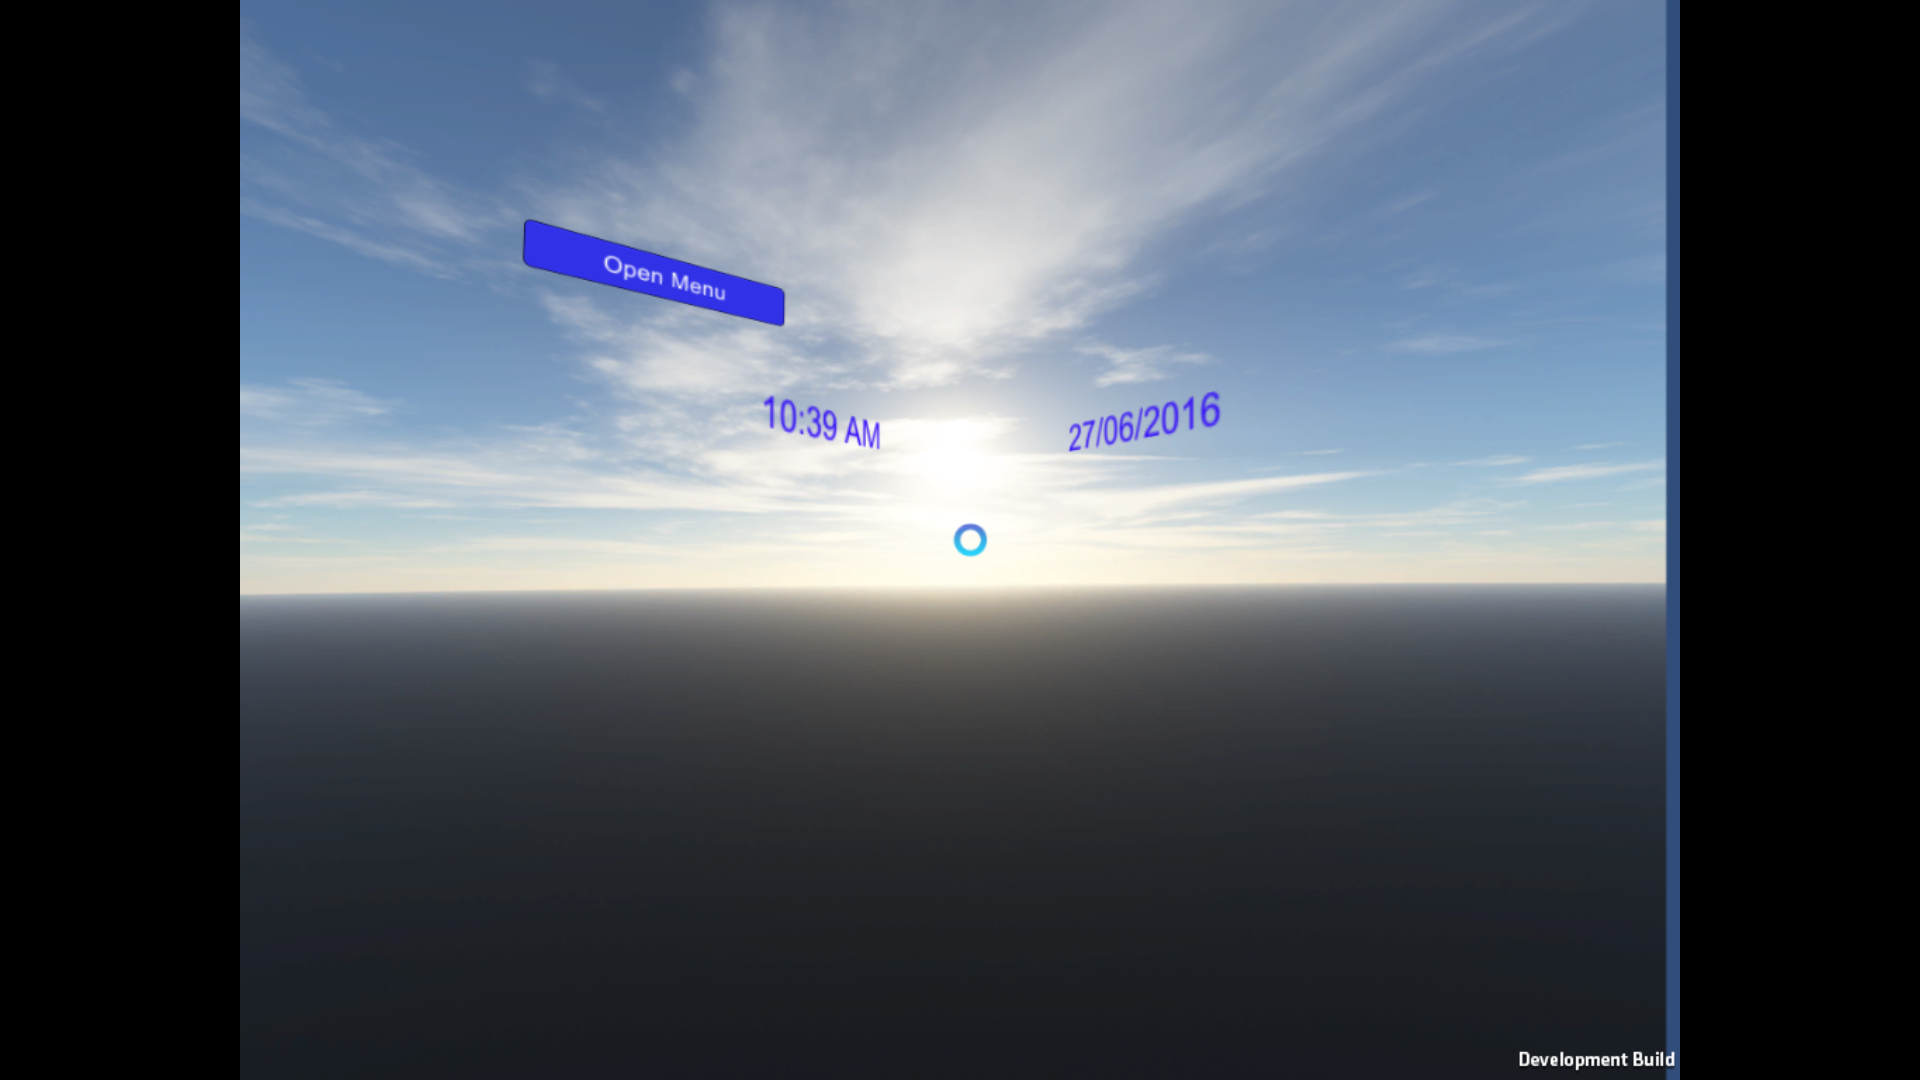
\includegraphics[width=\textwidth]{images/inicio.png} 
  \caption{Pantalla de inicio del sistema.}
  \label{fig:init2}
\end{figure}

\begin{figure} [H]
\centering	
	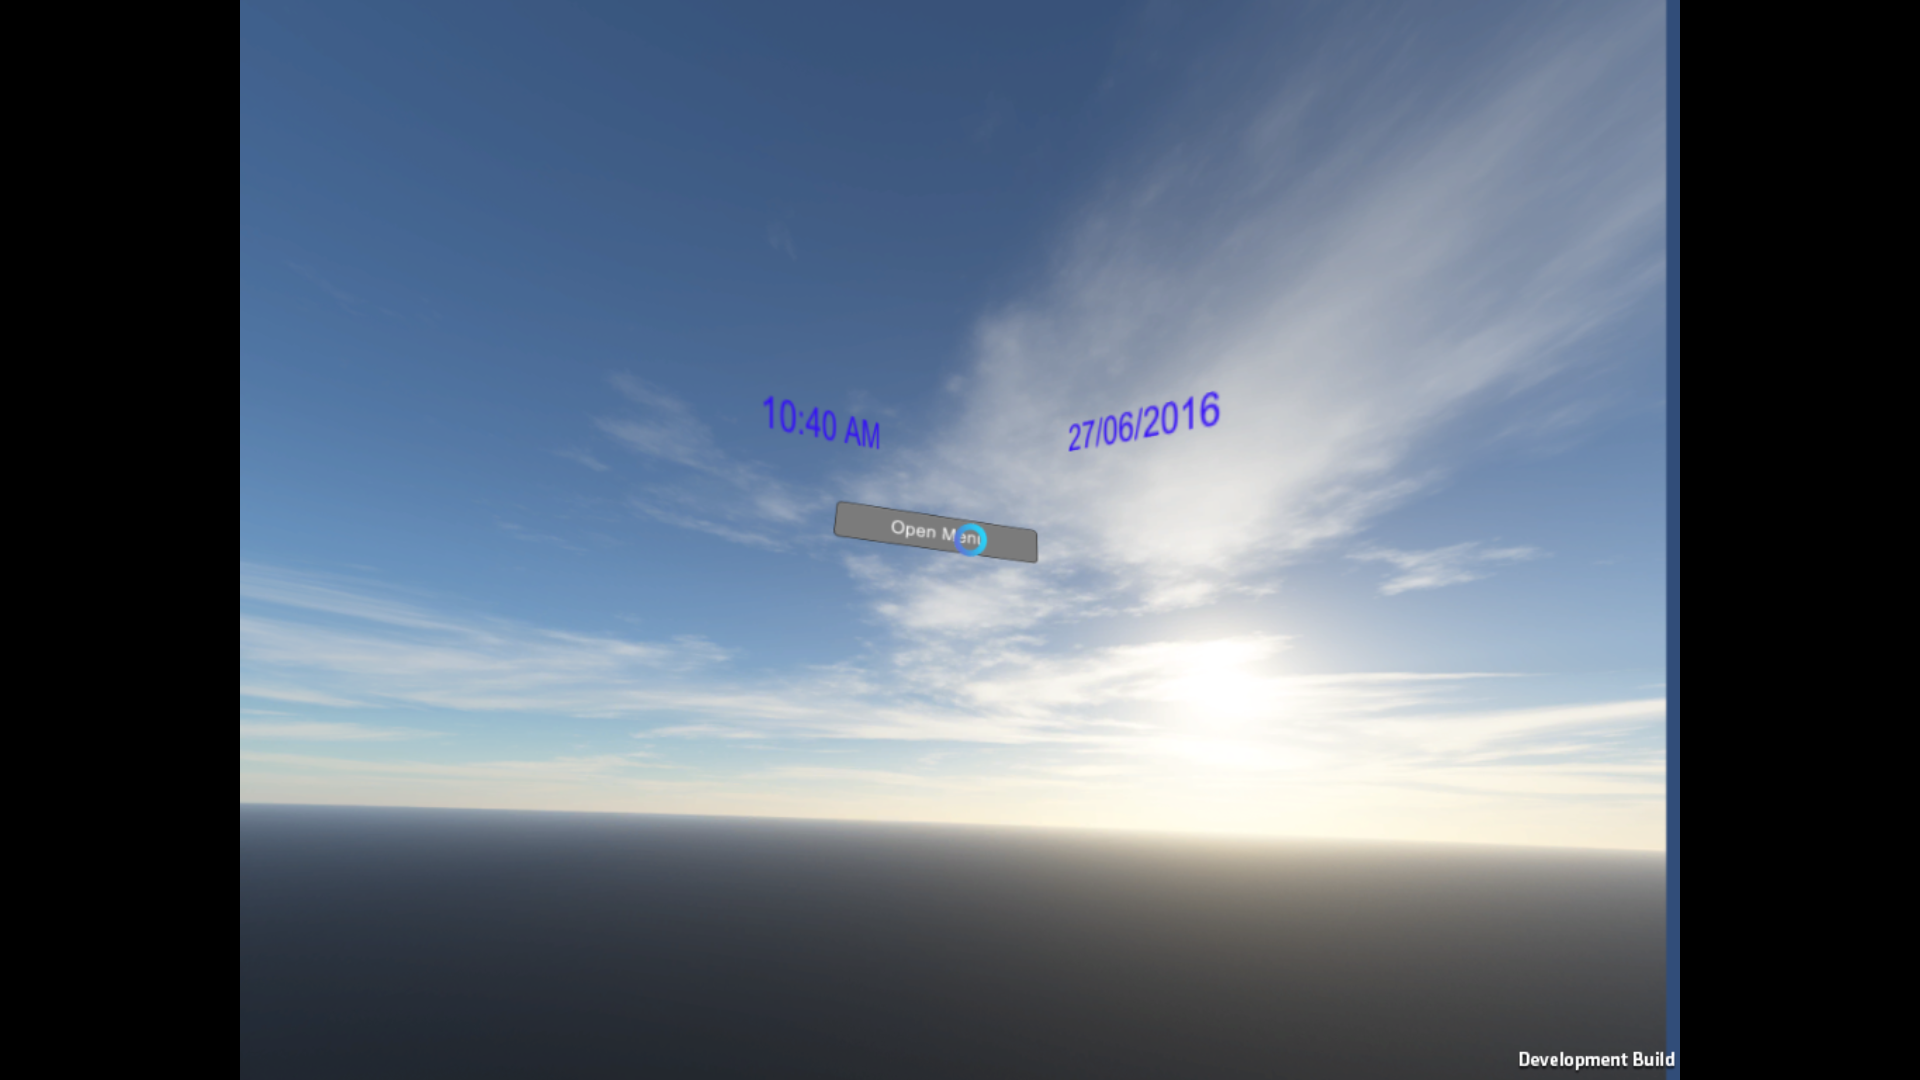
\includegraphics[width=\textwidth]{images/int_menu_open.png} 
  \caption{Usuario seleccionado la opci�n para abrir el men�.}
  \label{fig:openMenu2}
\end{figure}

\begin{figure} [H]
\centering	
	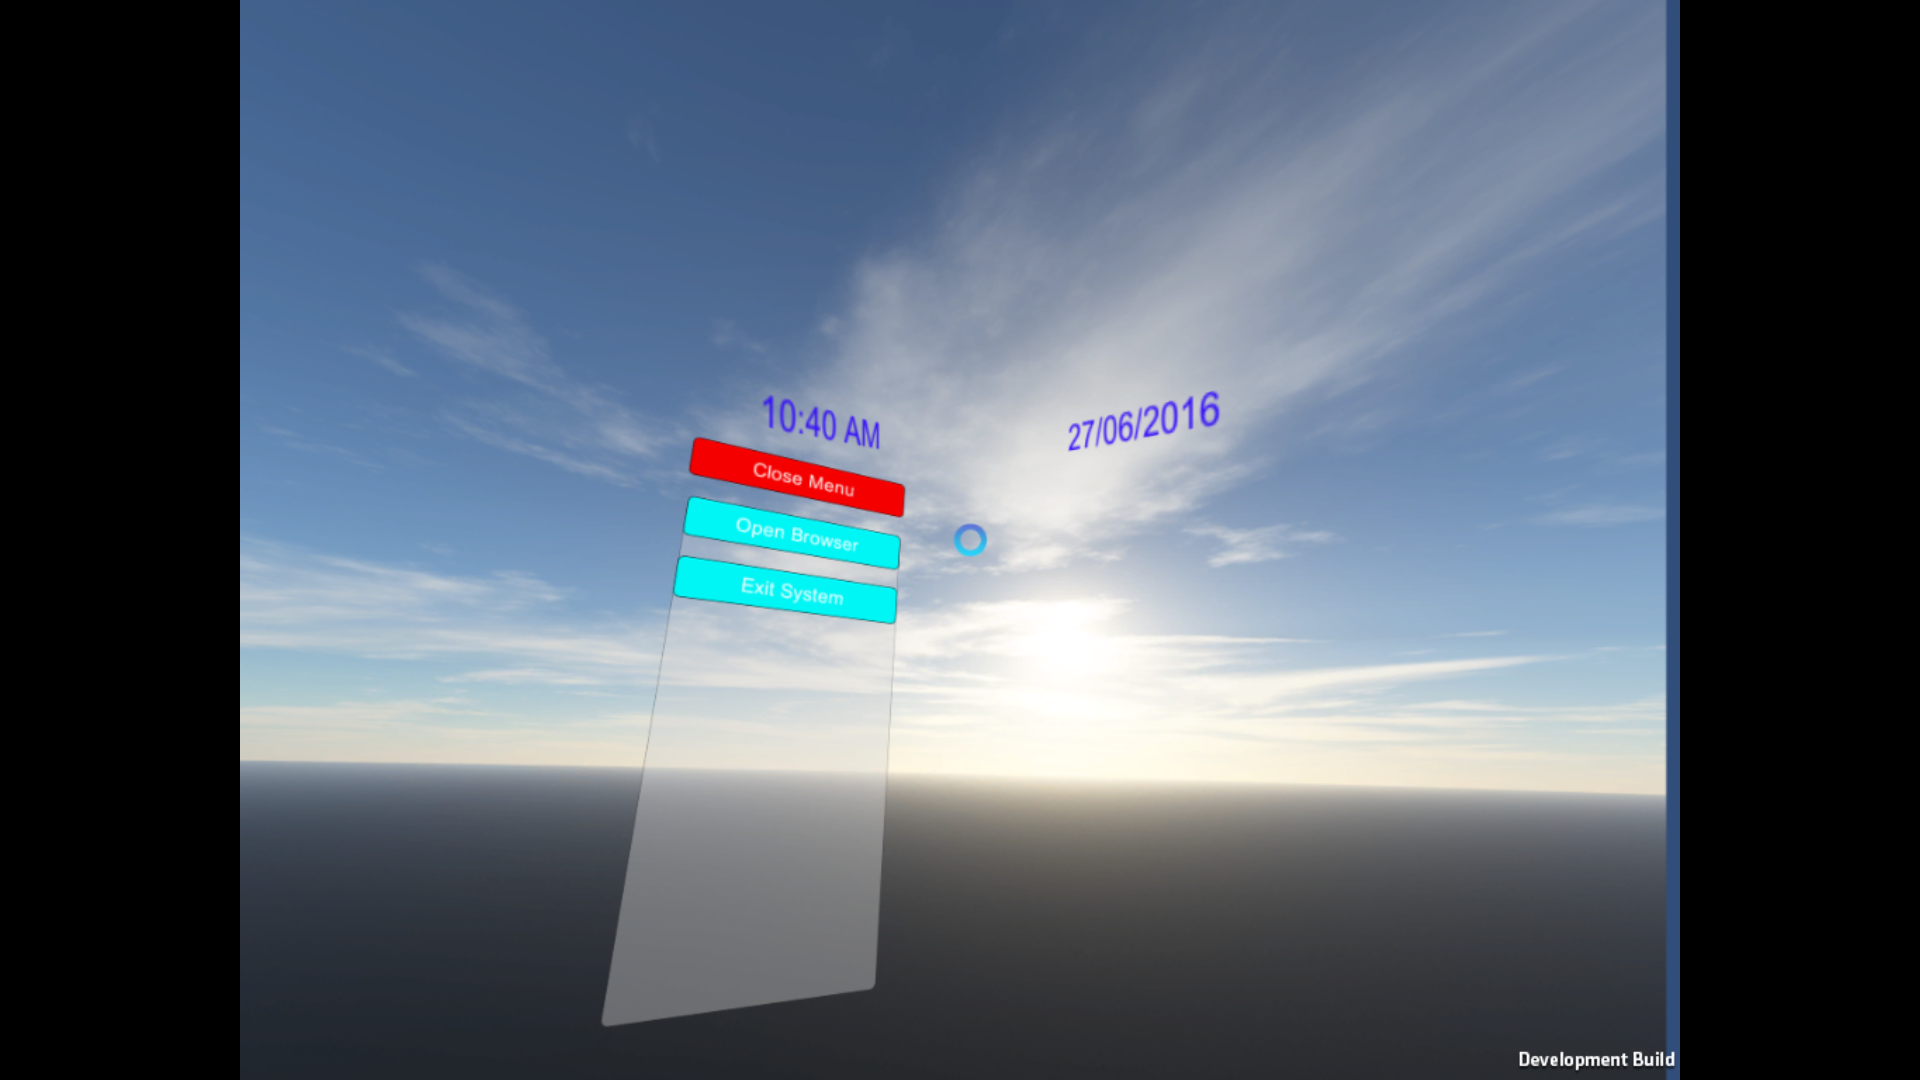
\includegraphics[width=\textwidth]{images/menu_abierto.png} 
  \caption{Men� desplegado.}
  \label{fig:menu2}
\end{figure}

\begin{figure} [H]
\centering	
	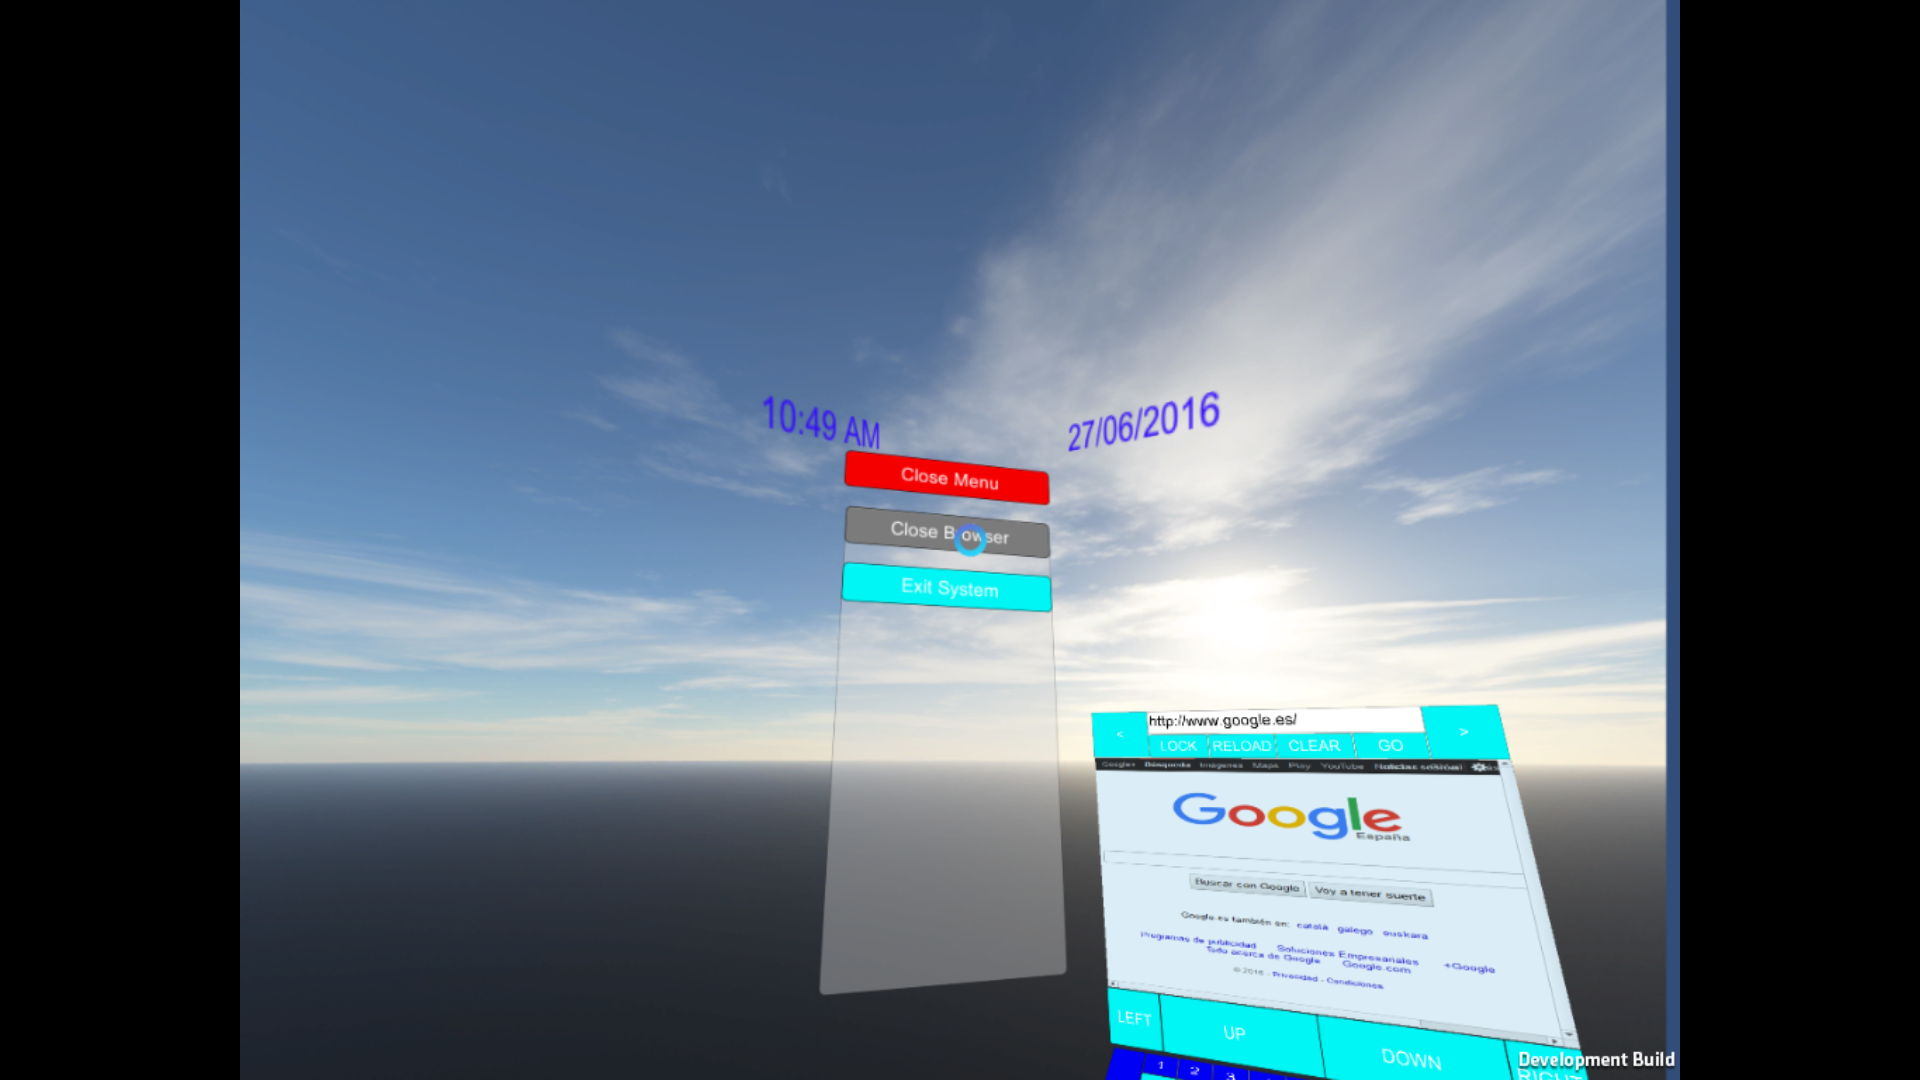
\includegraphics[width=\textwidth]{images/Apertura_browser.png} 
  \caption{Usuario seleccionando la opci�n para abrir el navegador.}
  \label{fig:initBrowser1}
\end{figure}

\begin{figure} [H]
\centering	
	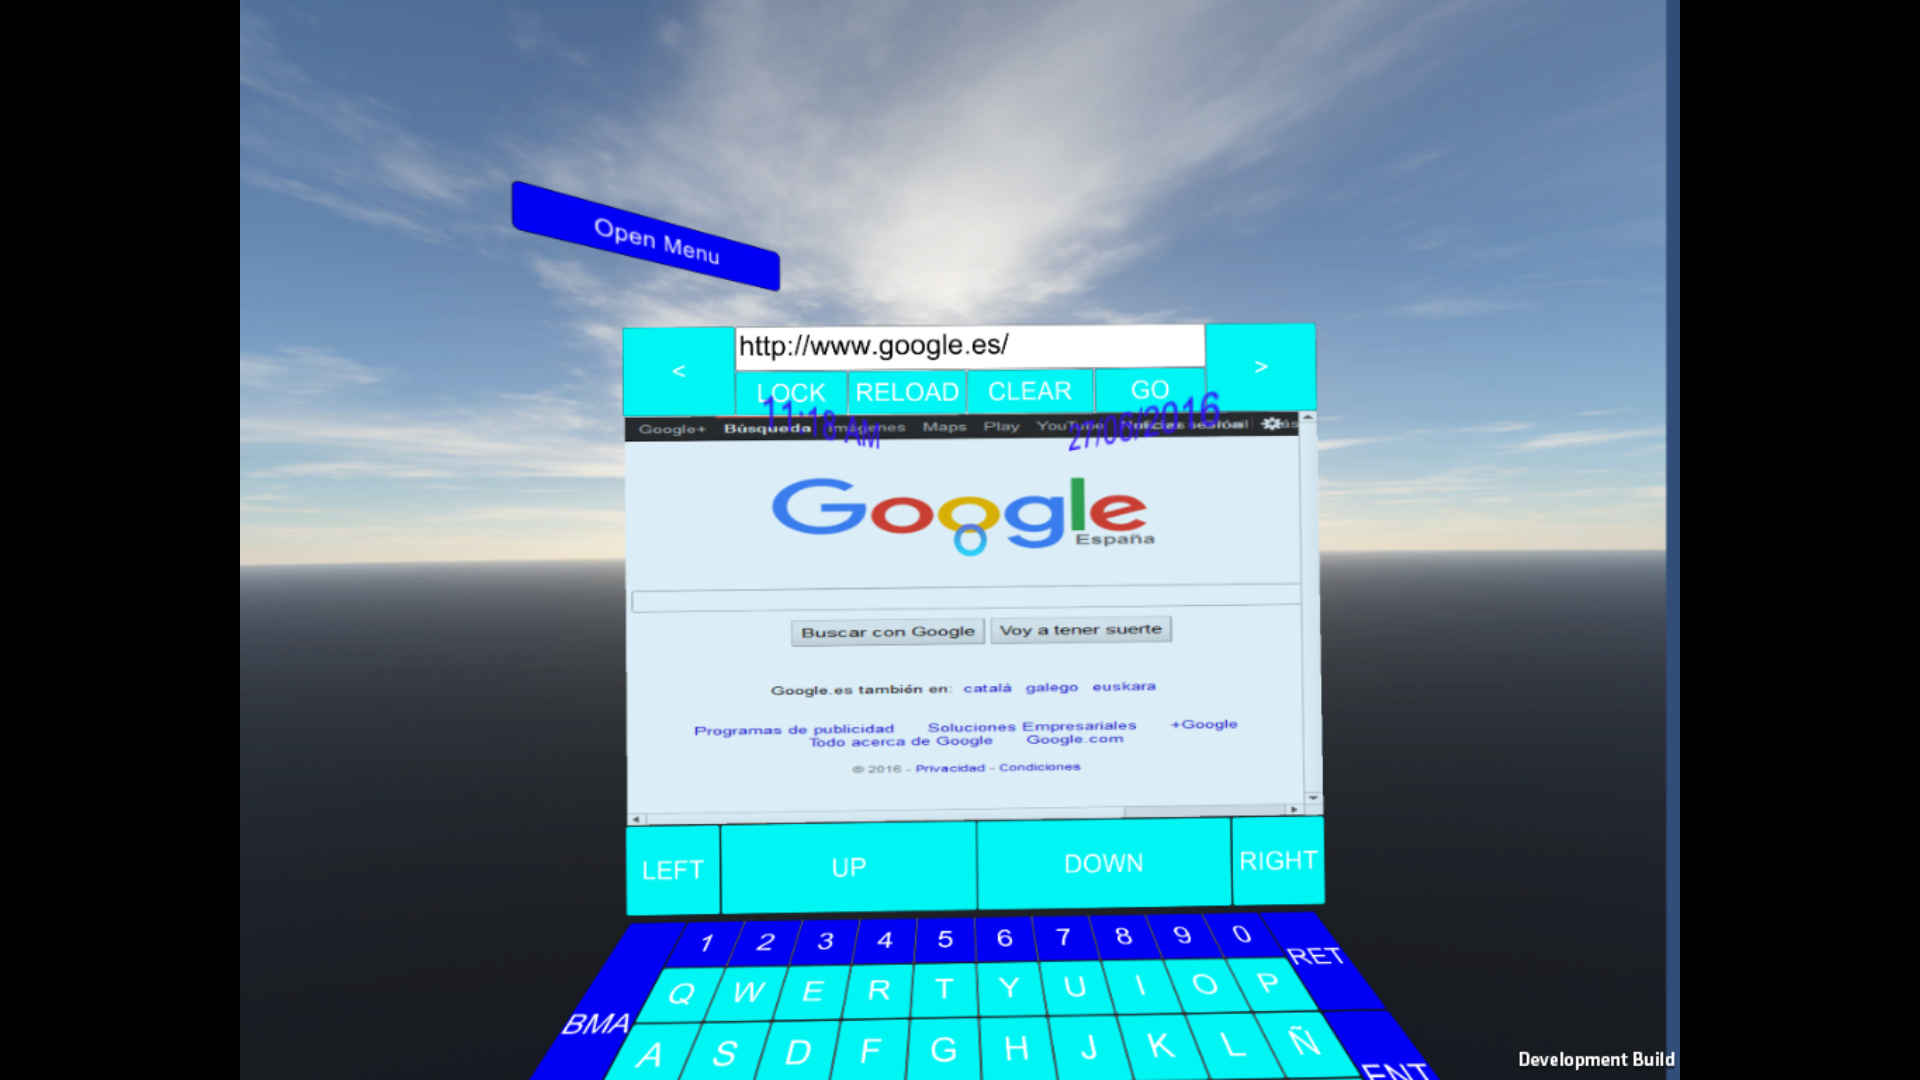
\includegraphics[width=\textwidth]{images/browser.png} 
  \caption{Navegador del sistema.}
  \label{fig:browser1}
\end{figure}


\begin{figure} [H]
\centering	
	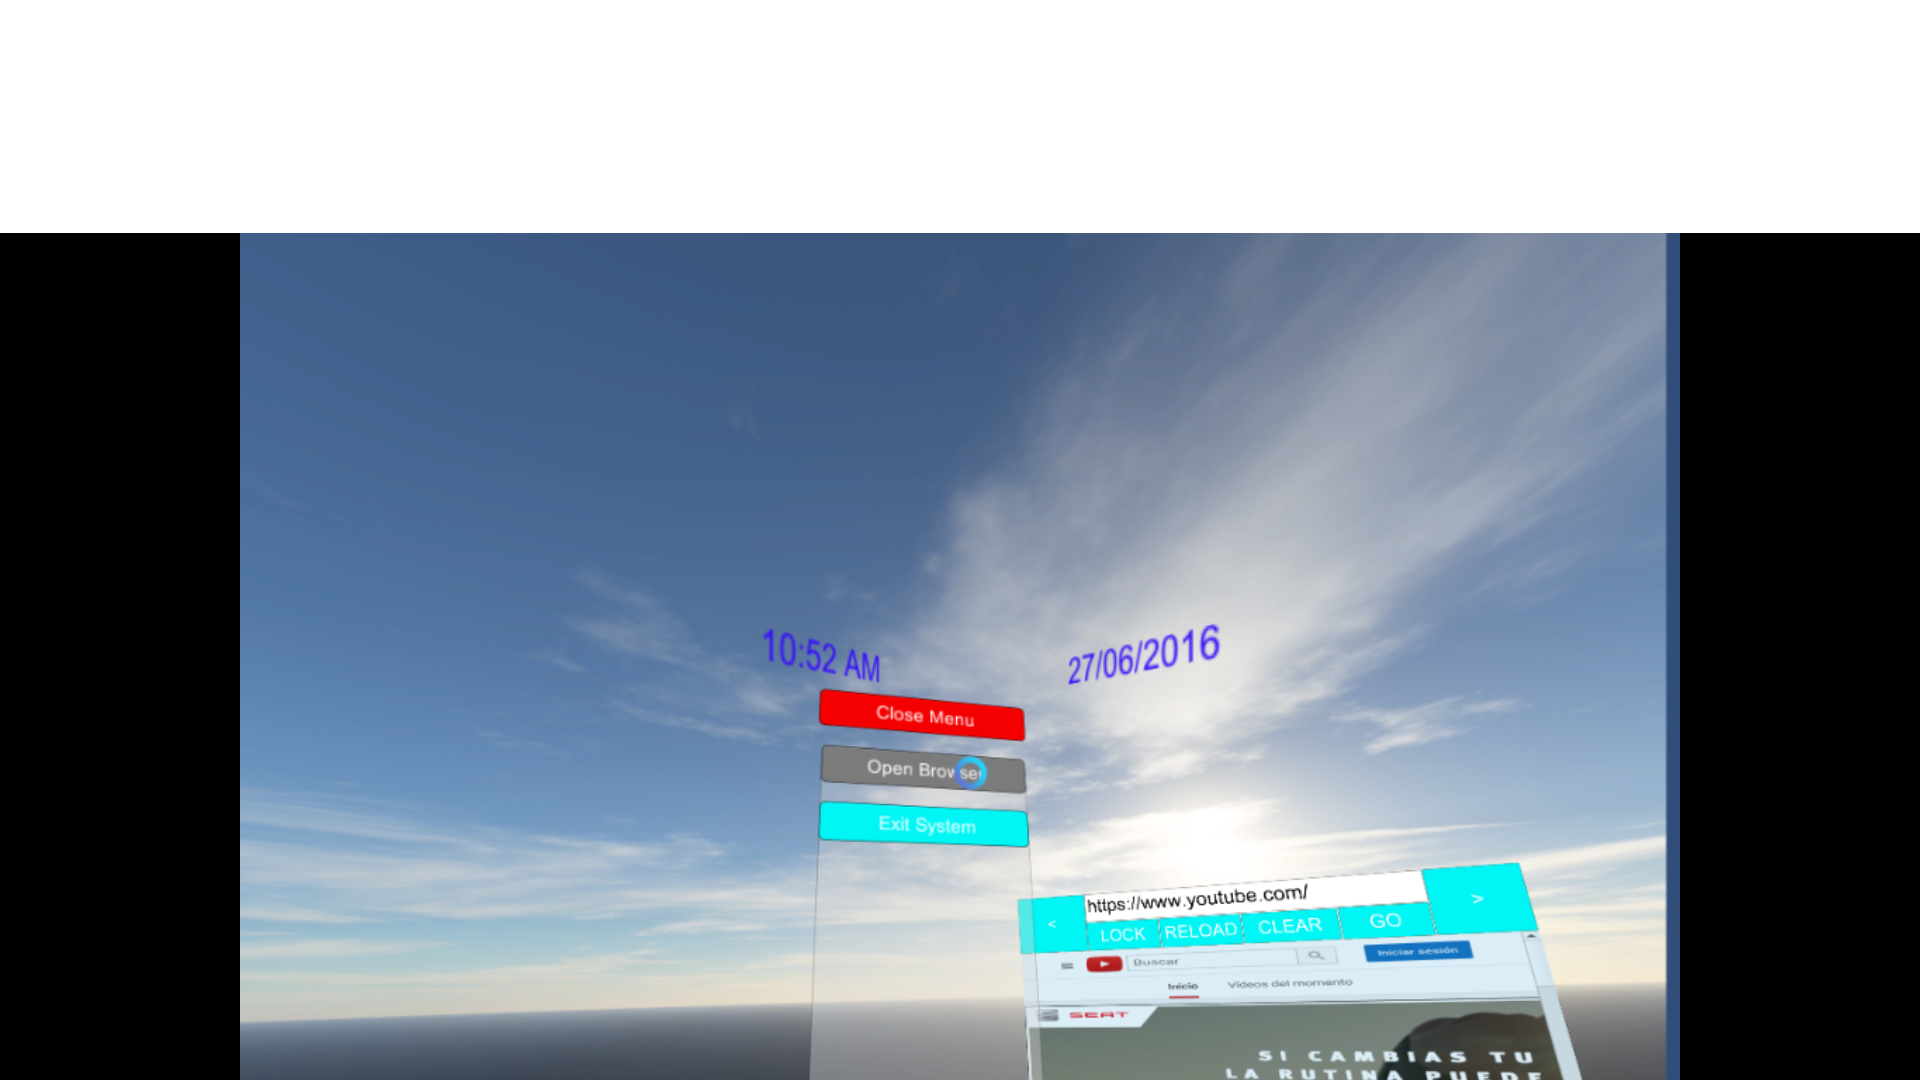
\includegraphics[width=\textwidth]{images/cierre_navegador.png} 
  \caption{Usuario seleccionado la opci�n para cerrar el navegador.}
  \label{fig:exitBrowser1}
\end{figure}

\begin{figure} [H]
\centering	
	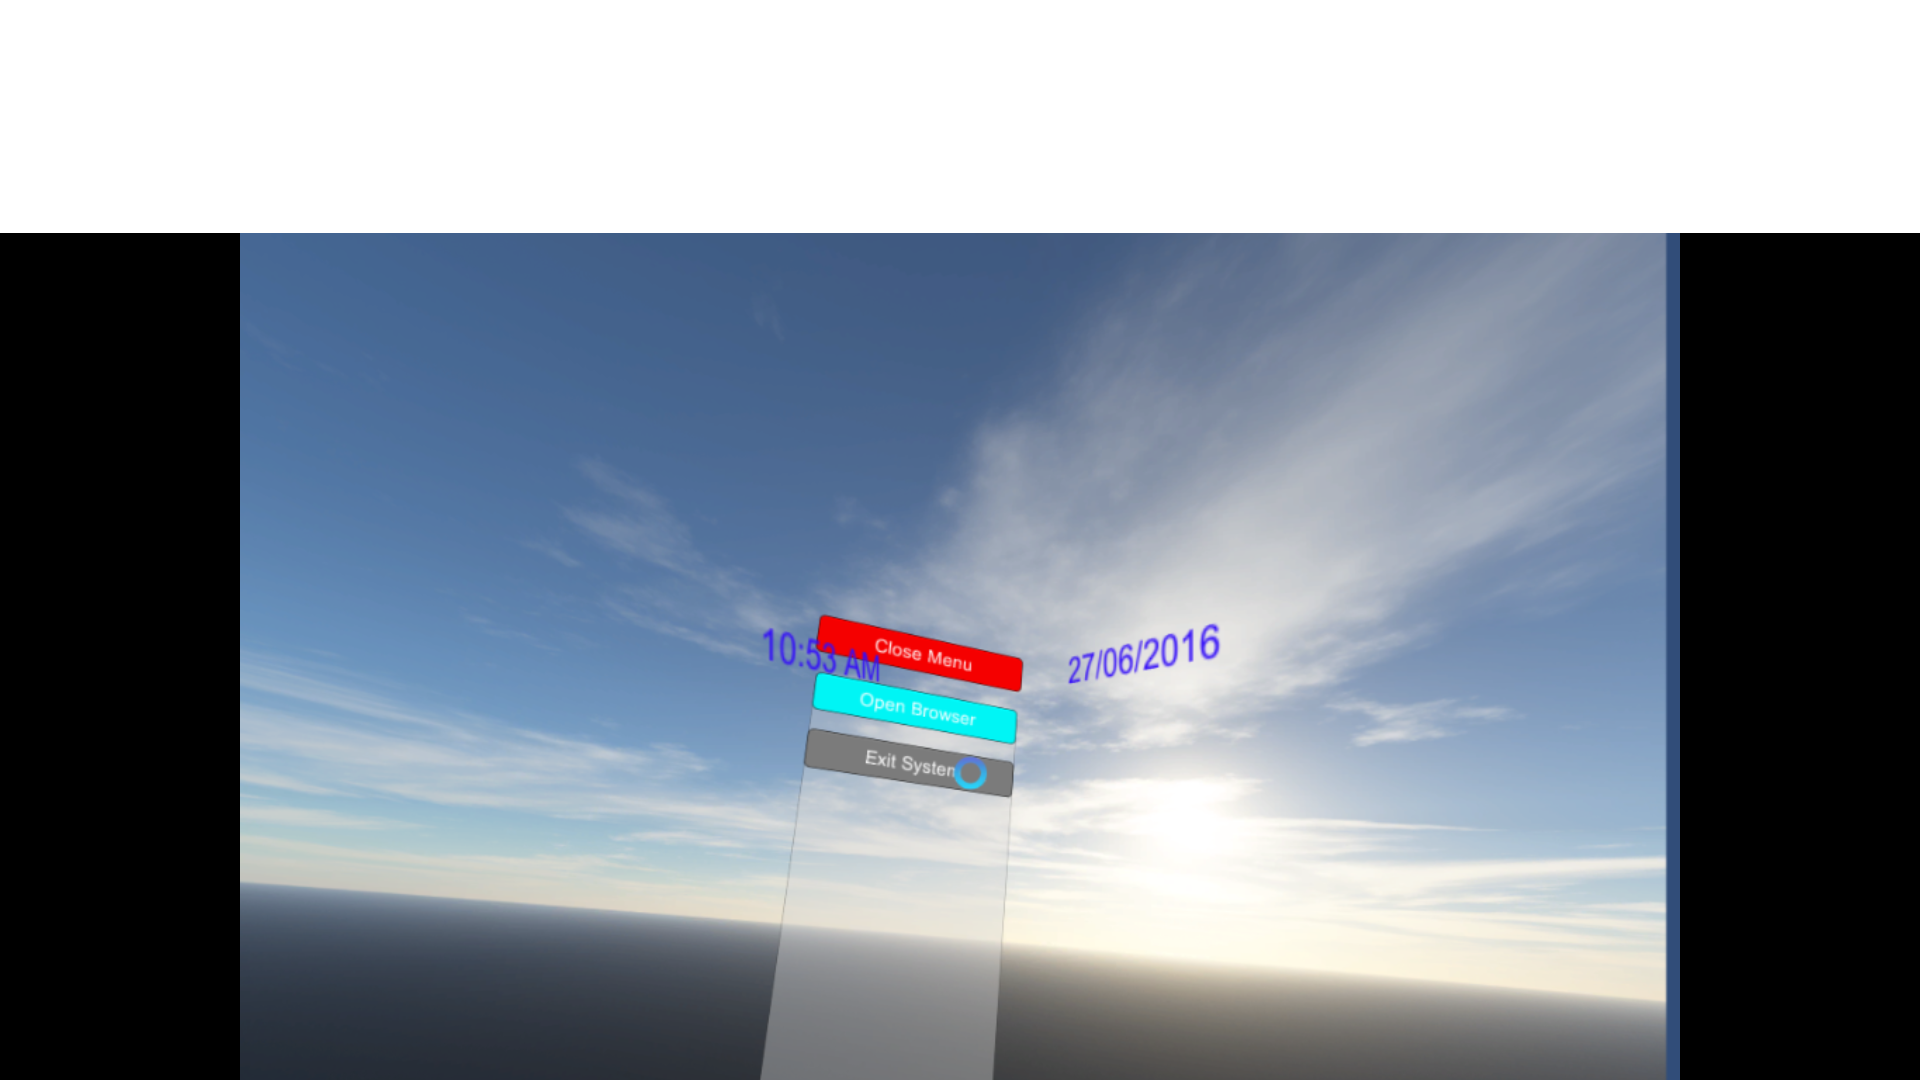
\includegraphics[width=\textwidth]{images/salir_sistema.png} 
  \caption{Usuario seleccionado la opci�n para apagar el sistema}
  \label{fig:exit2}
\end{figure}

\lsection{Caso 3}
\label{Anexo:caso3}
Recordemos este caso de uso. El usuario debe abrir el men� desplegable y seleccionar la opci�n del navegador. A posterior� debe introducir la URL \url{www.youtube.es}, cargar la p�gina, seleccionar el primer v�deo que aparezca y cerrar todo el sistema.

\begin{figure} [H]
\centering	
	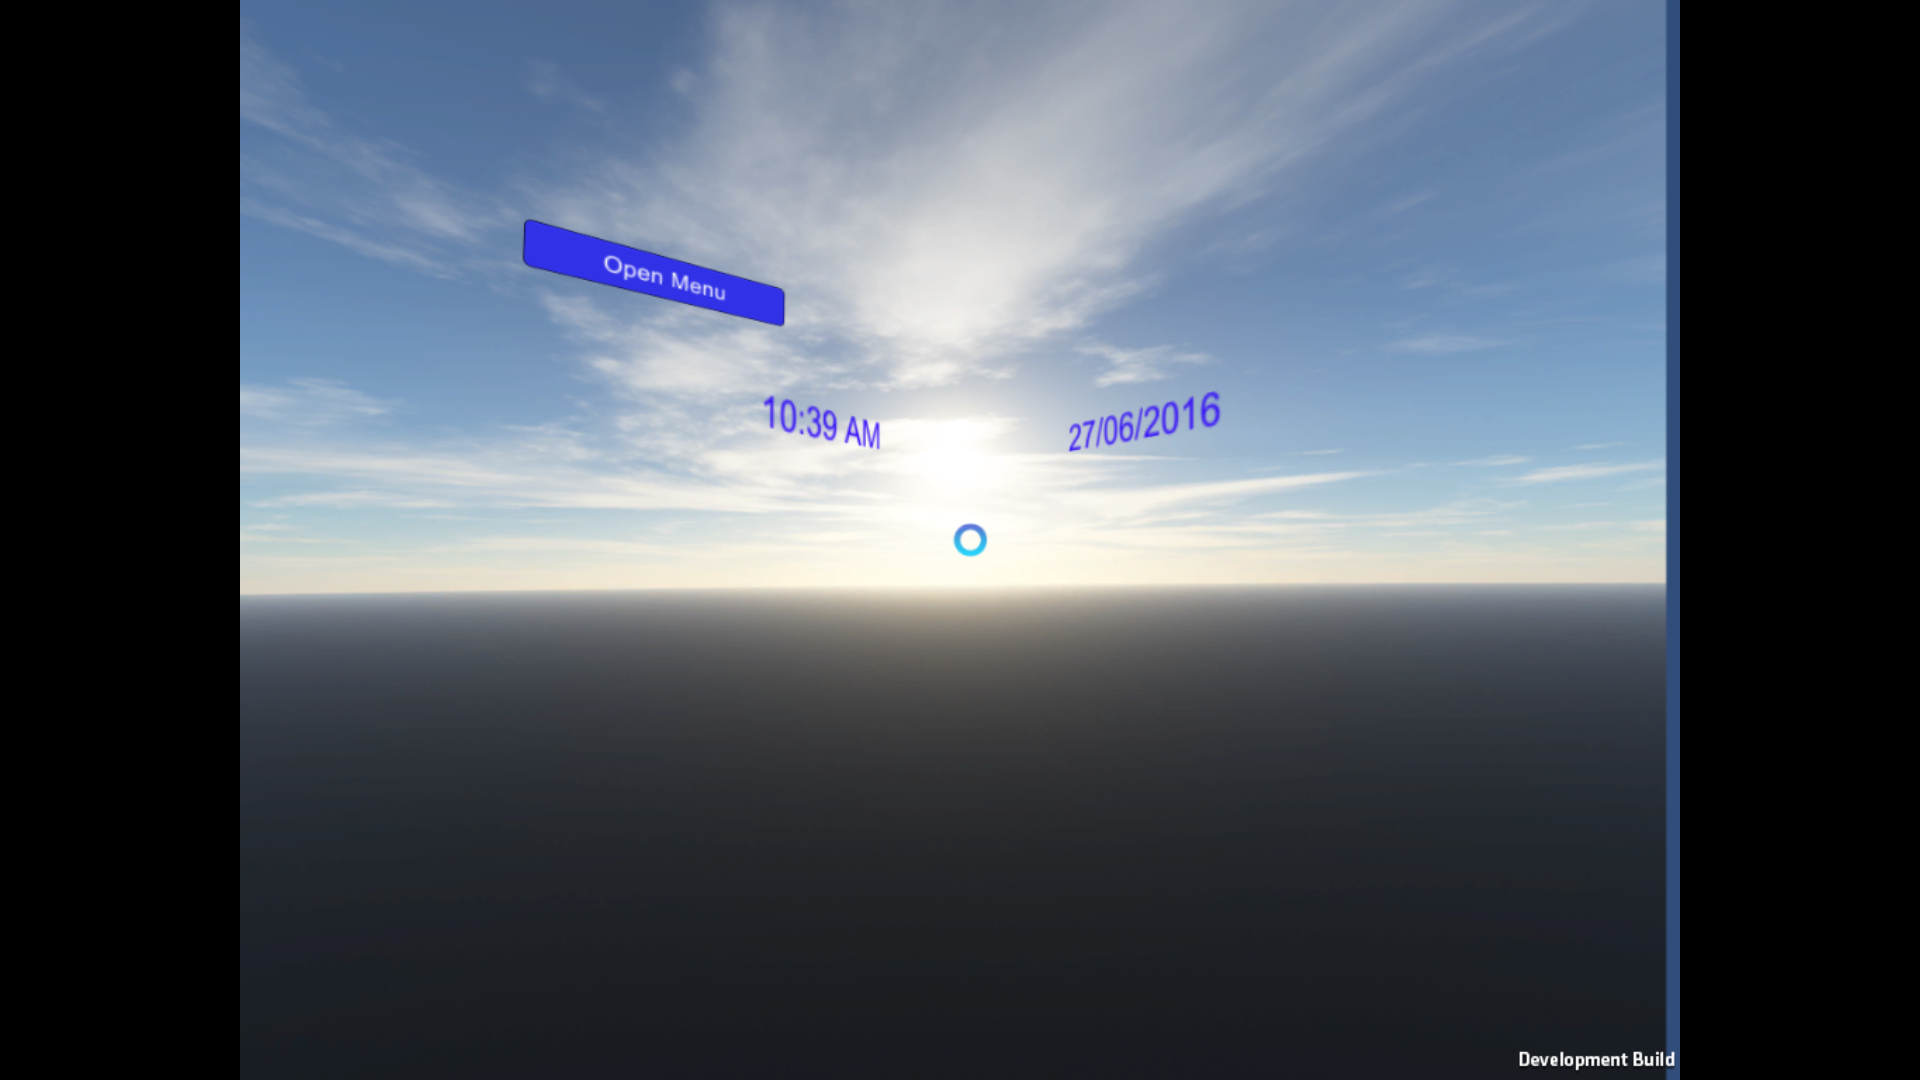
\includegraphics[width=\textwidth]{images/inicio.png} 
  \caption{Pantalla de inicio del sistema.}
  \label{fig:init3}
\end{figure}

\begin{figure} [H]
\centering	
	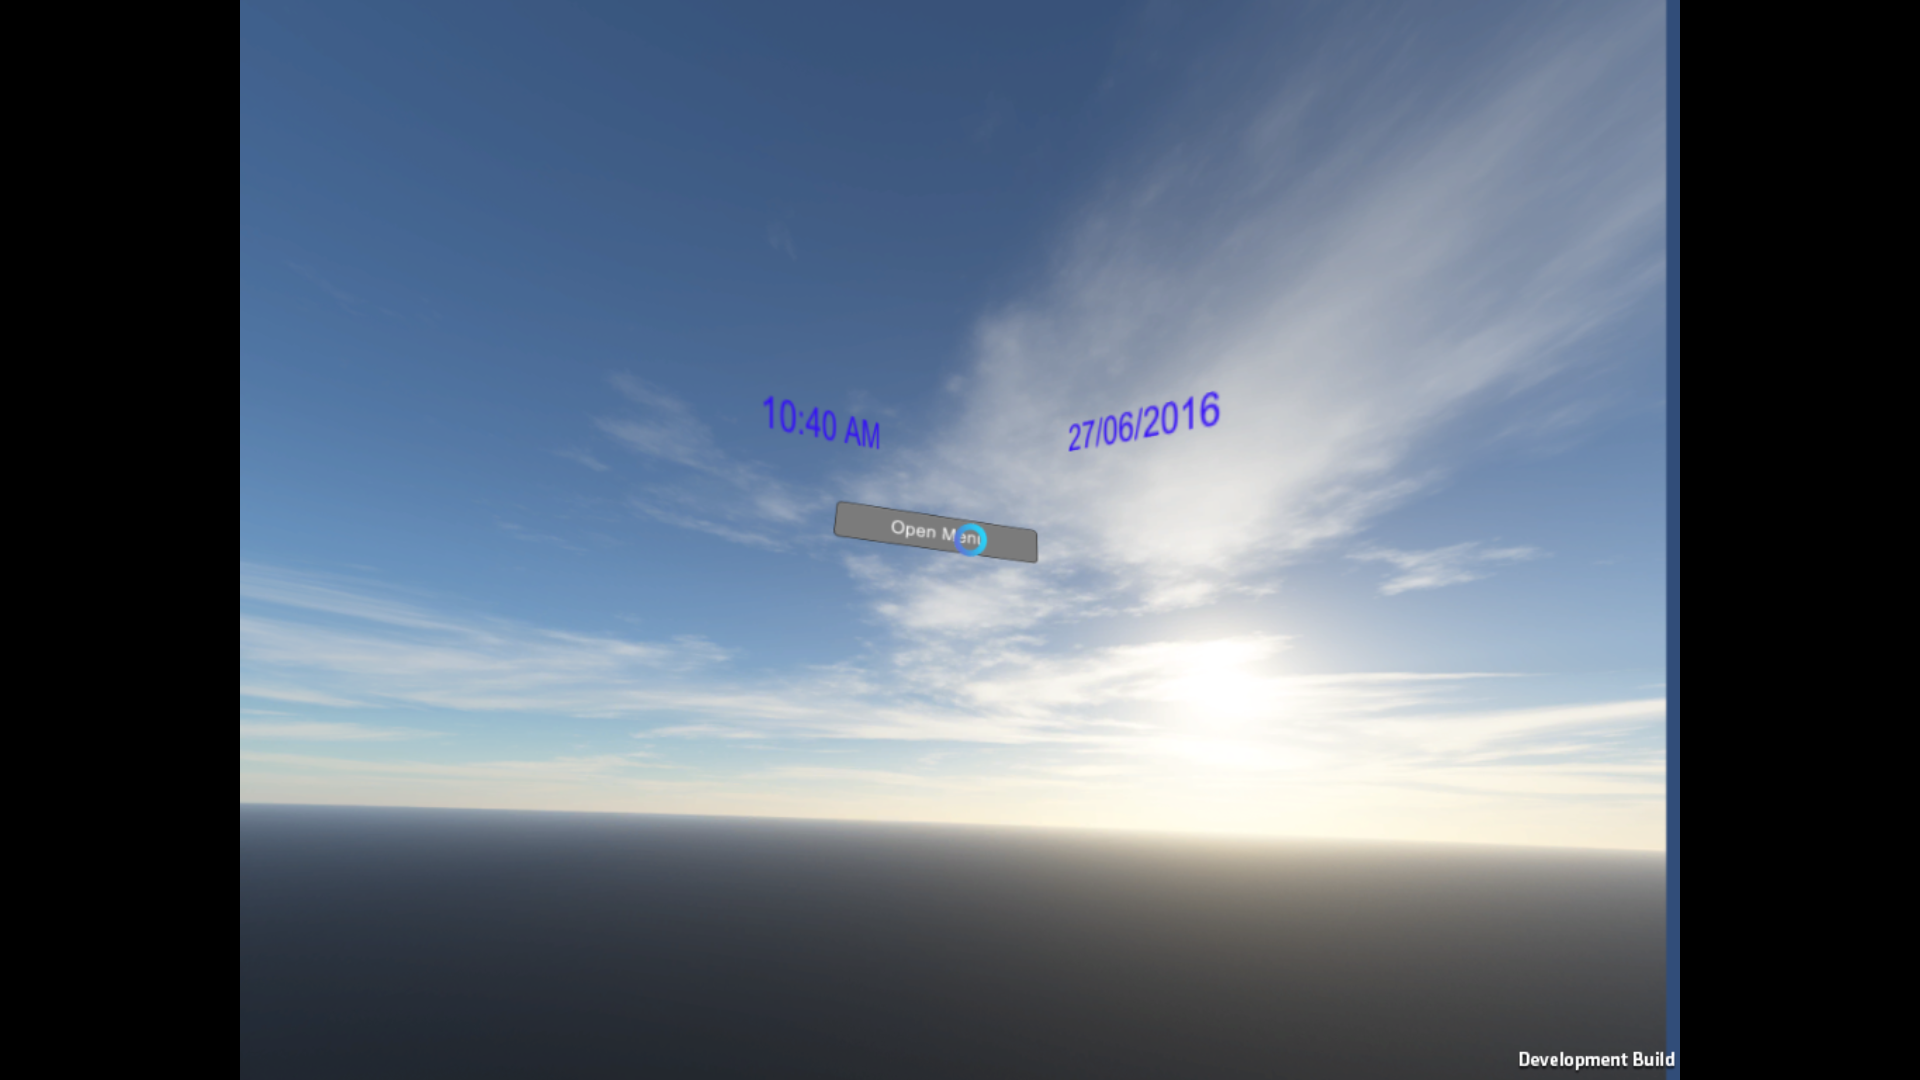
\includegraphics[width=\textwidth]{images/int_menu_open.png} 
  \caption{Usuario seleccionado la opci�n para abrir el men�.}
  \label{fig:openMenu3}
\end{figure}

\begin{figure} [H]
\centering	
	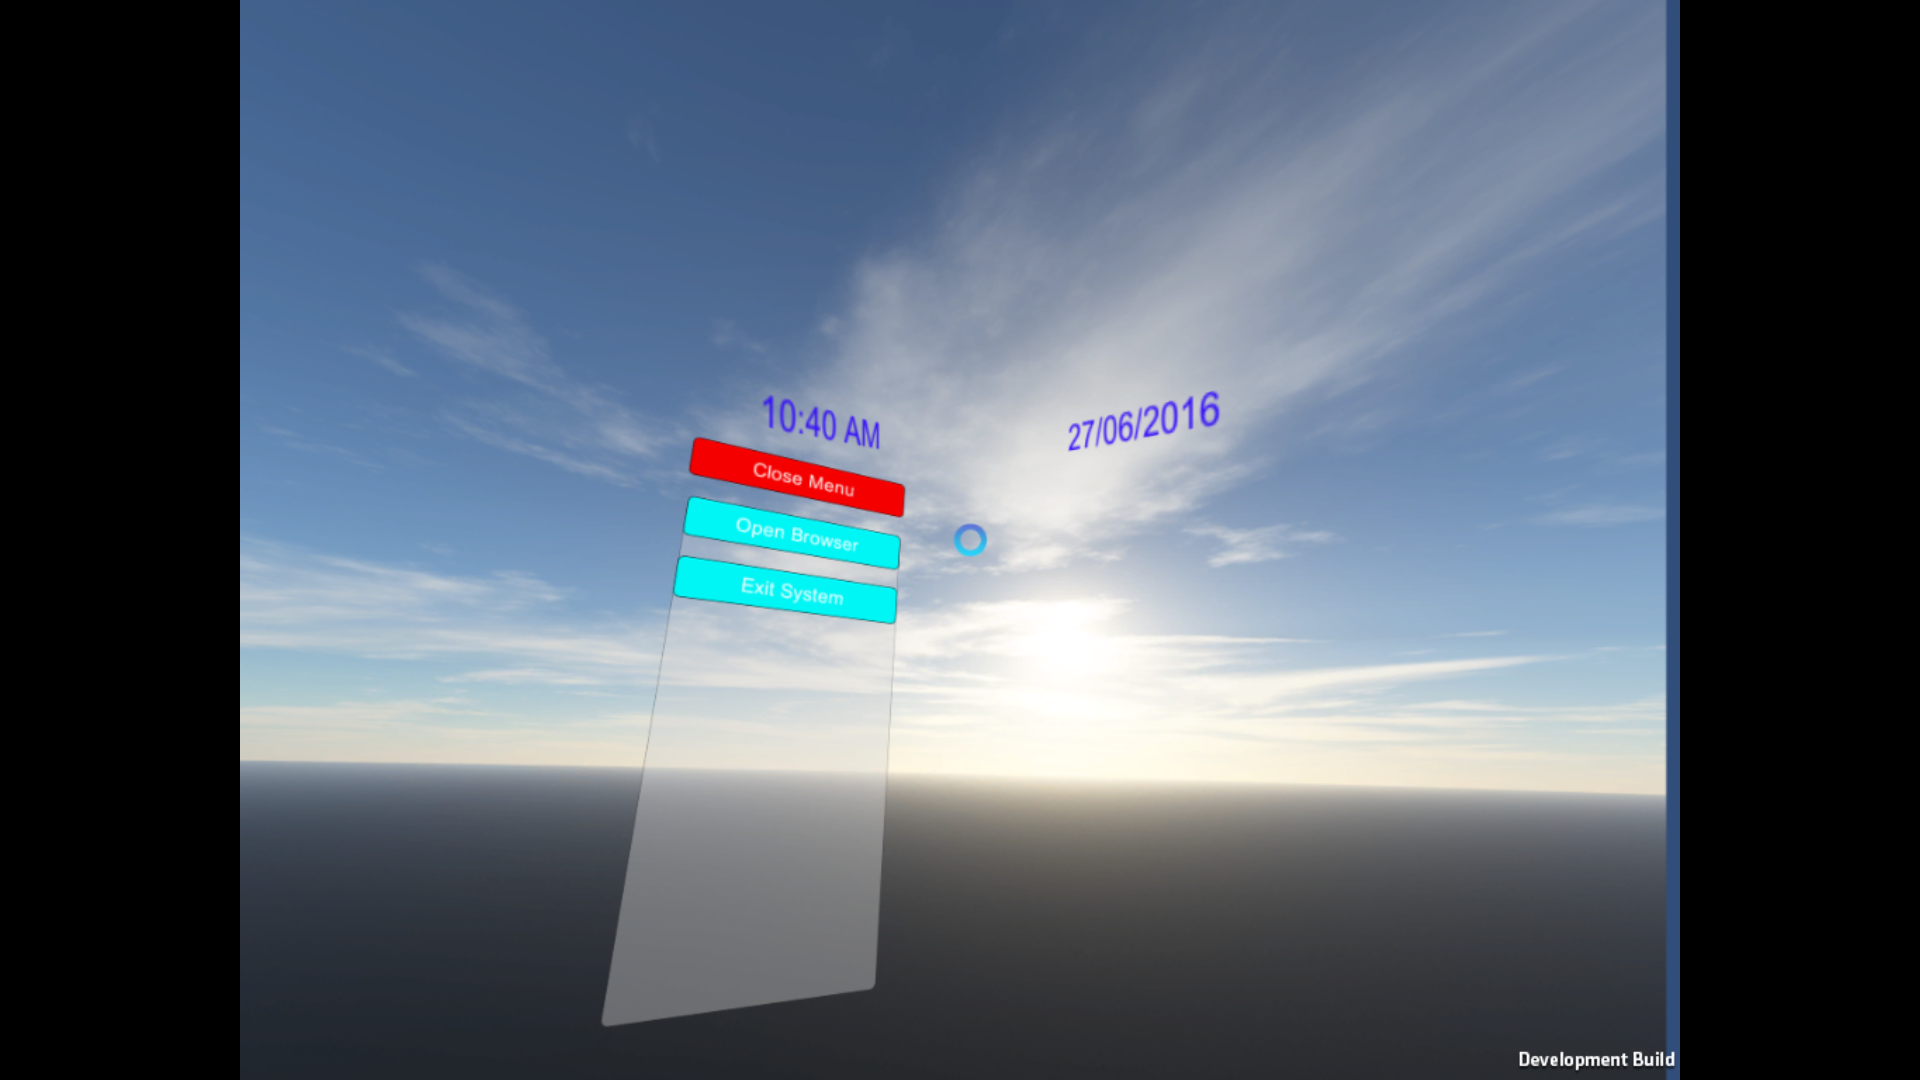
\includegraphics[width=\textwidth]{images/menu_abierto.png} 
  \caption{Men� desplegado.}
  \label{fig:menu3}
\end{figure}

\begin{figure} [H]
\centering	
	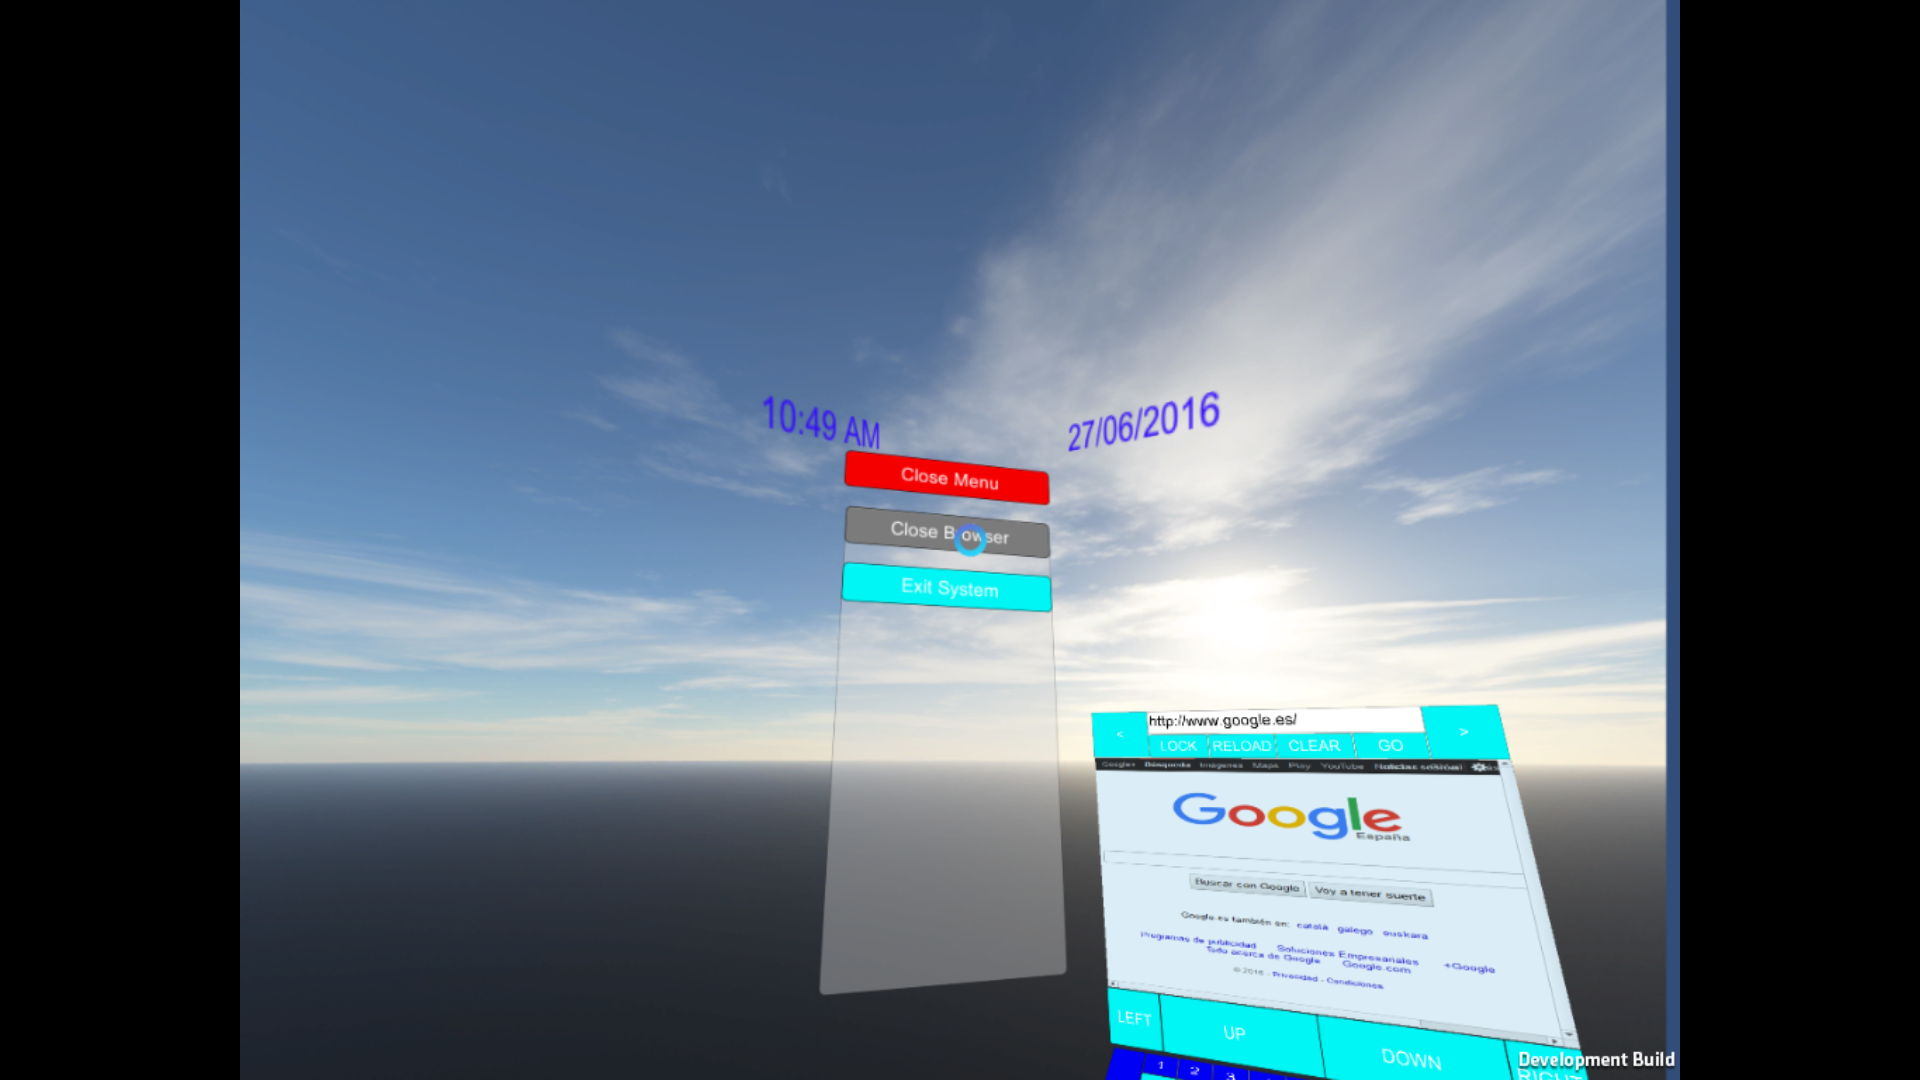
\includegraphics[width=\textwidth]{images/Apertura_browser.png} 
  \caption{Usuario seleccionando la opci�n para abrir el navegador.}
  \label{fig:initBrowser2}
\end{figure}

\begin{figure} [H]
\centering	
	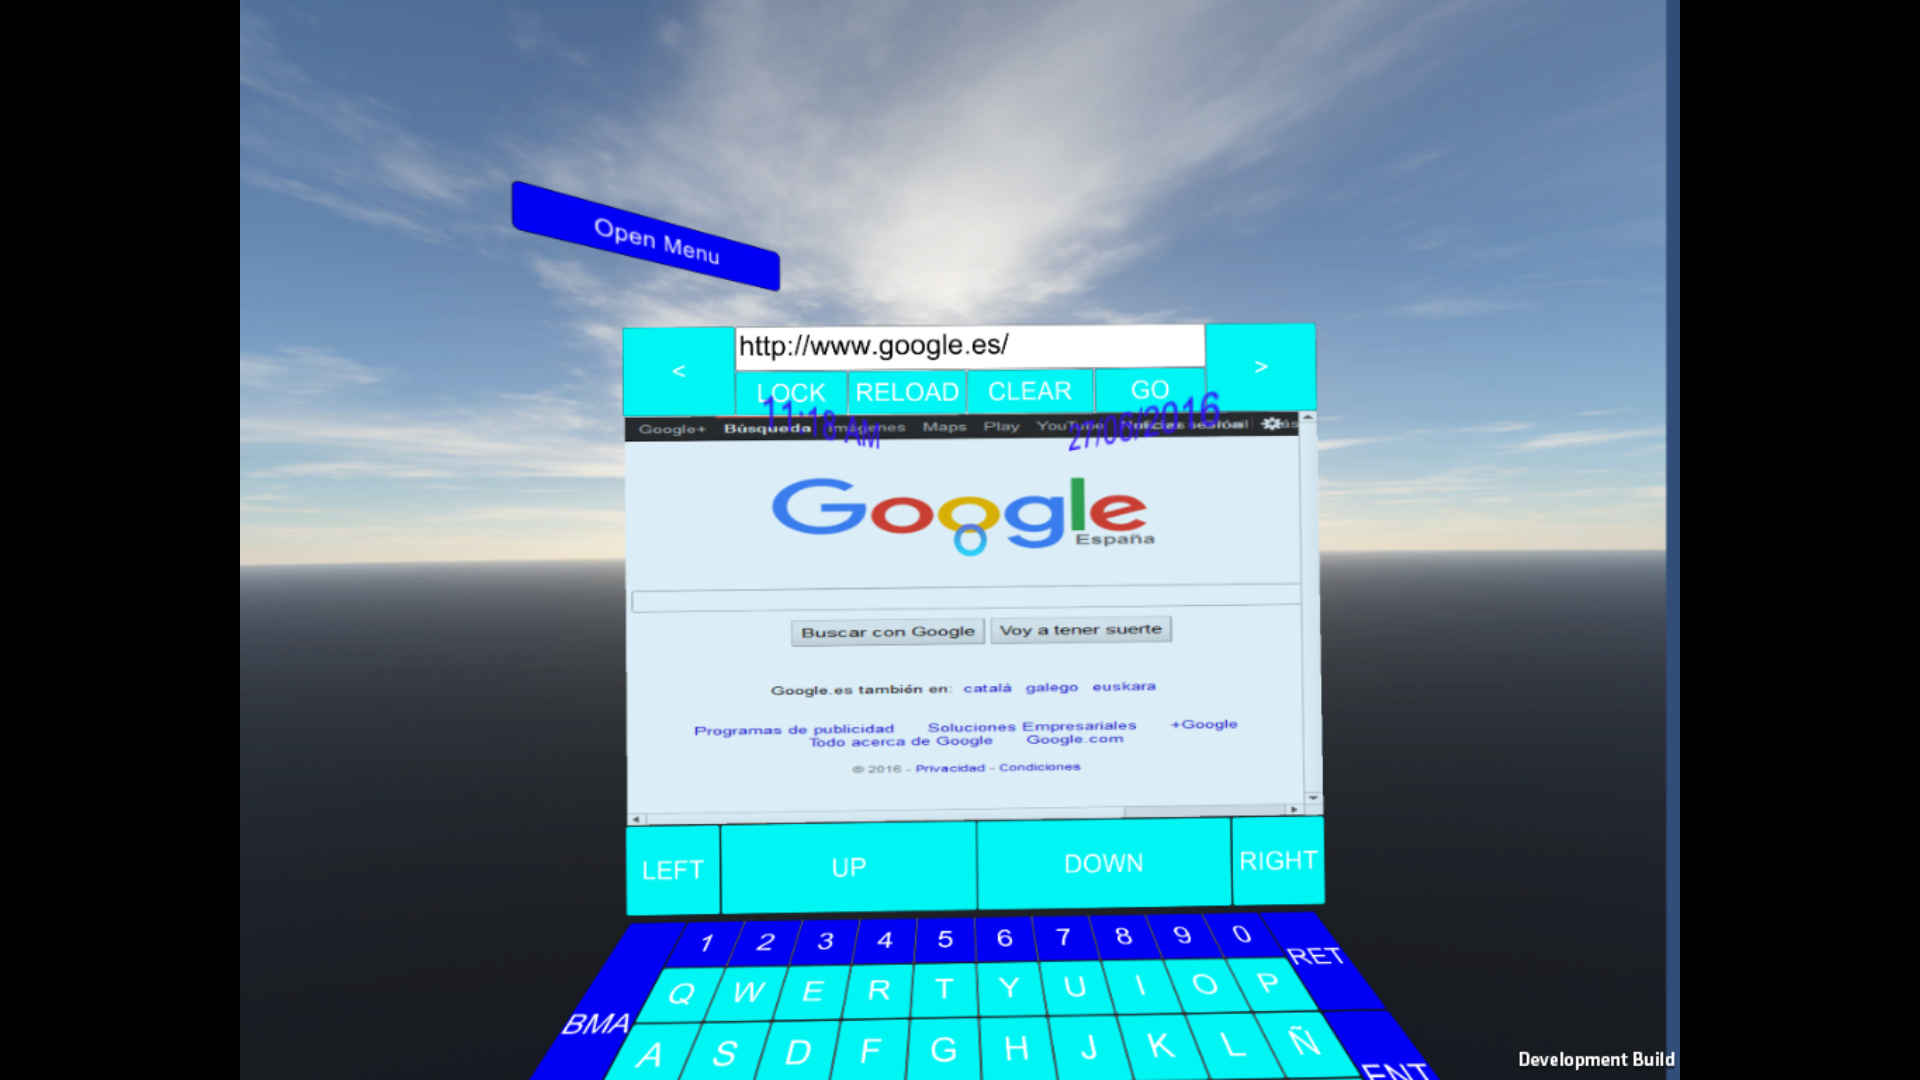
\includegraphics[width=\textwidth]{images/browser.png} 
  \caption{Navegador del sistema.}
  \label{fig:browser2}
\end{figure}

\begin{figure} [H]
\centering	
	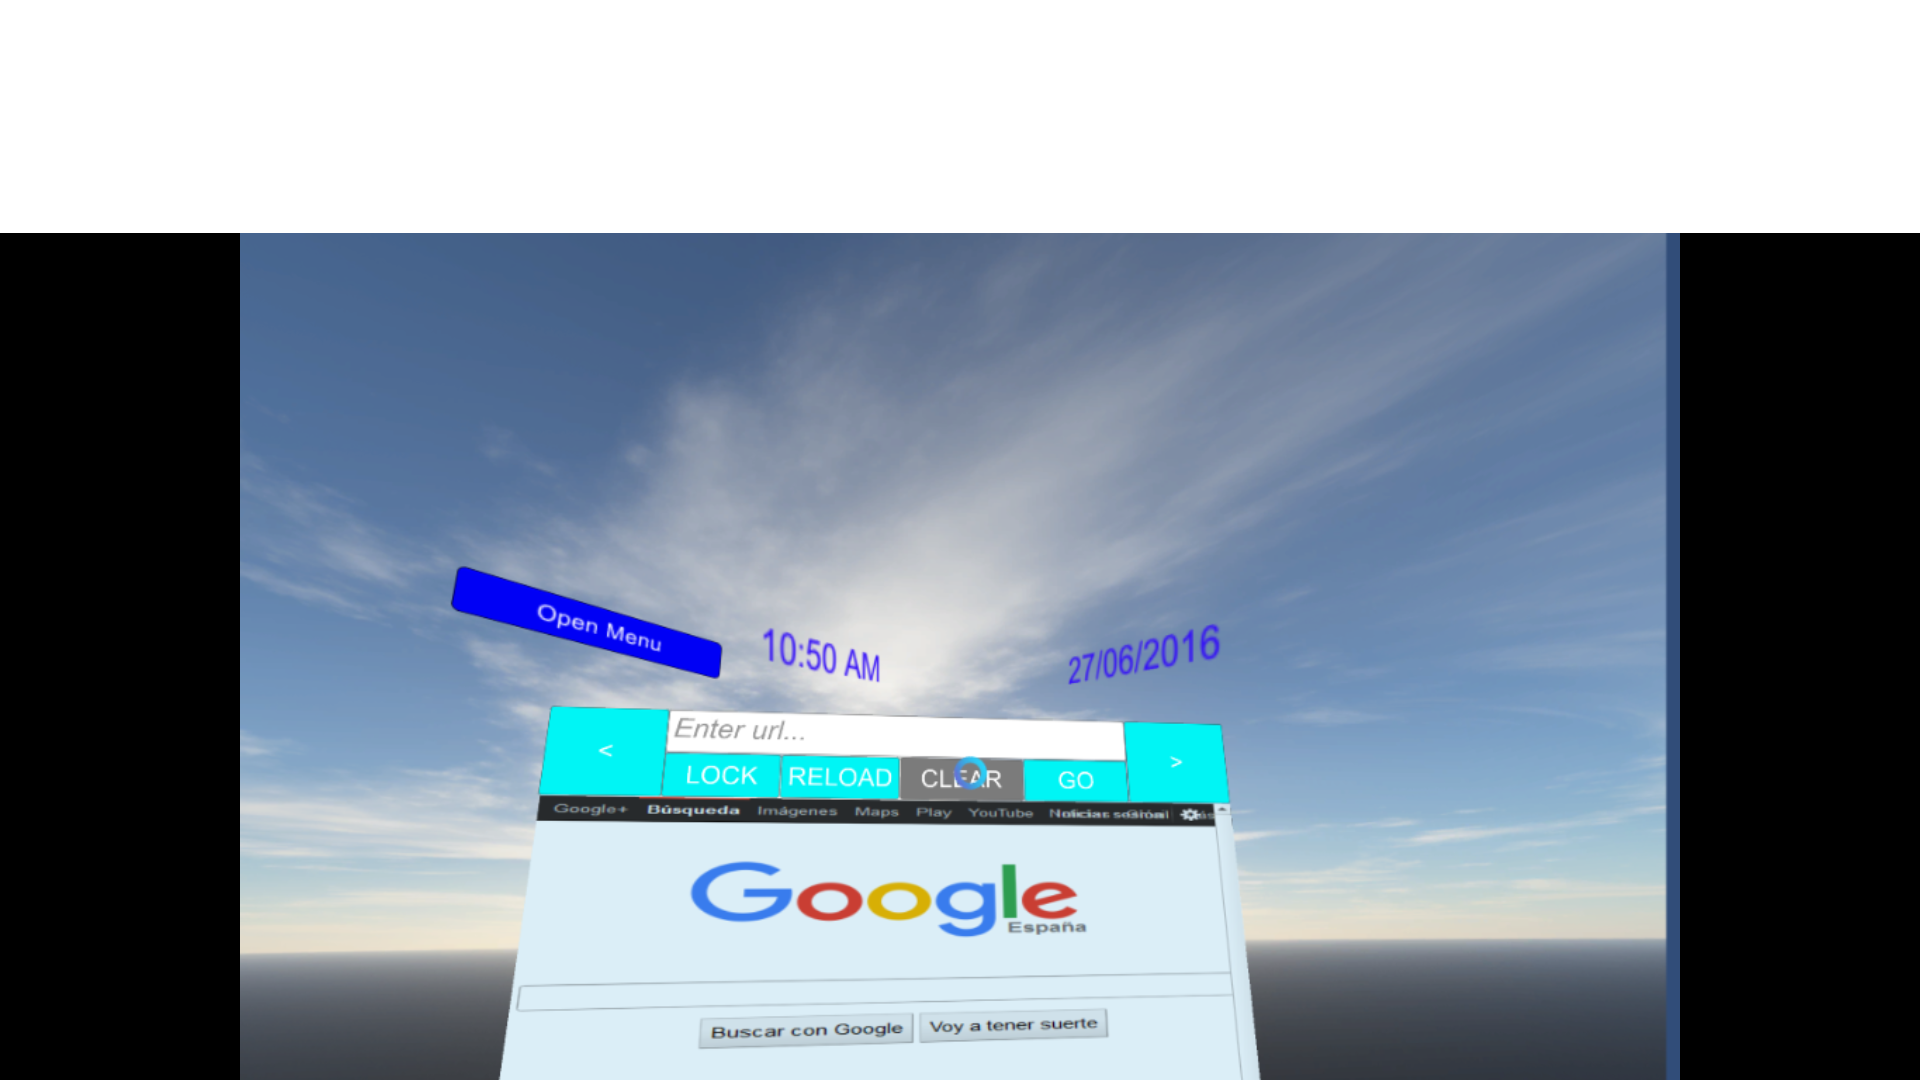
\includegraphics[width=\textwidth]{images/limpia_url.png} 
  \caption{Limpiando campo para escribir la URL.}
  \label{fig:urlClean1}
\end{figure}

\begin{figure} [H]
\centering	
	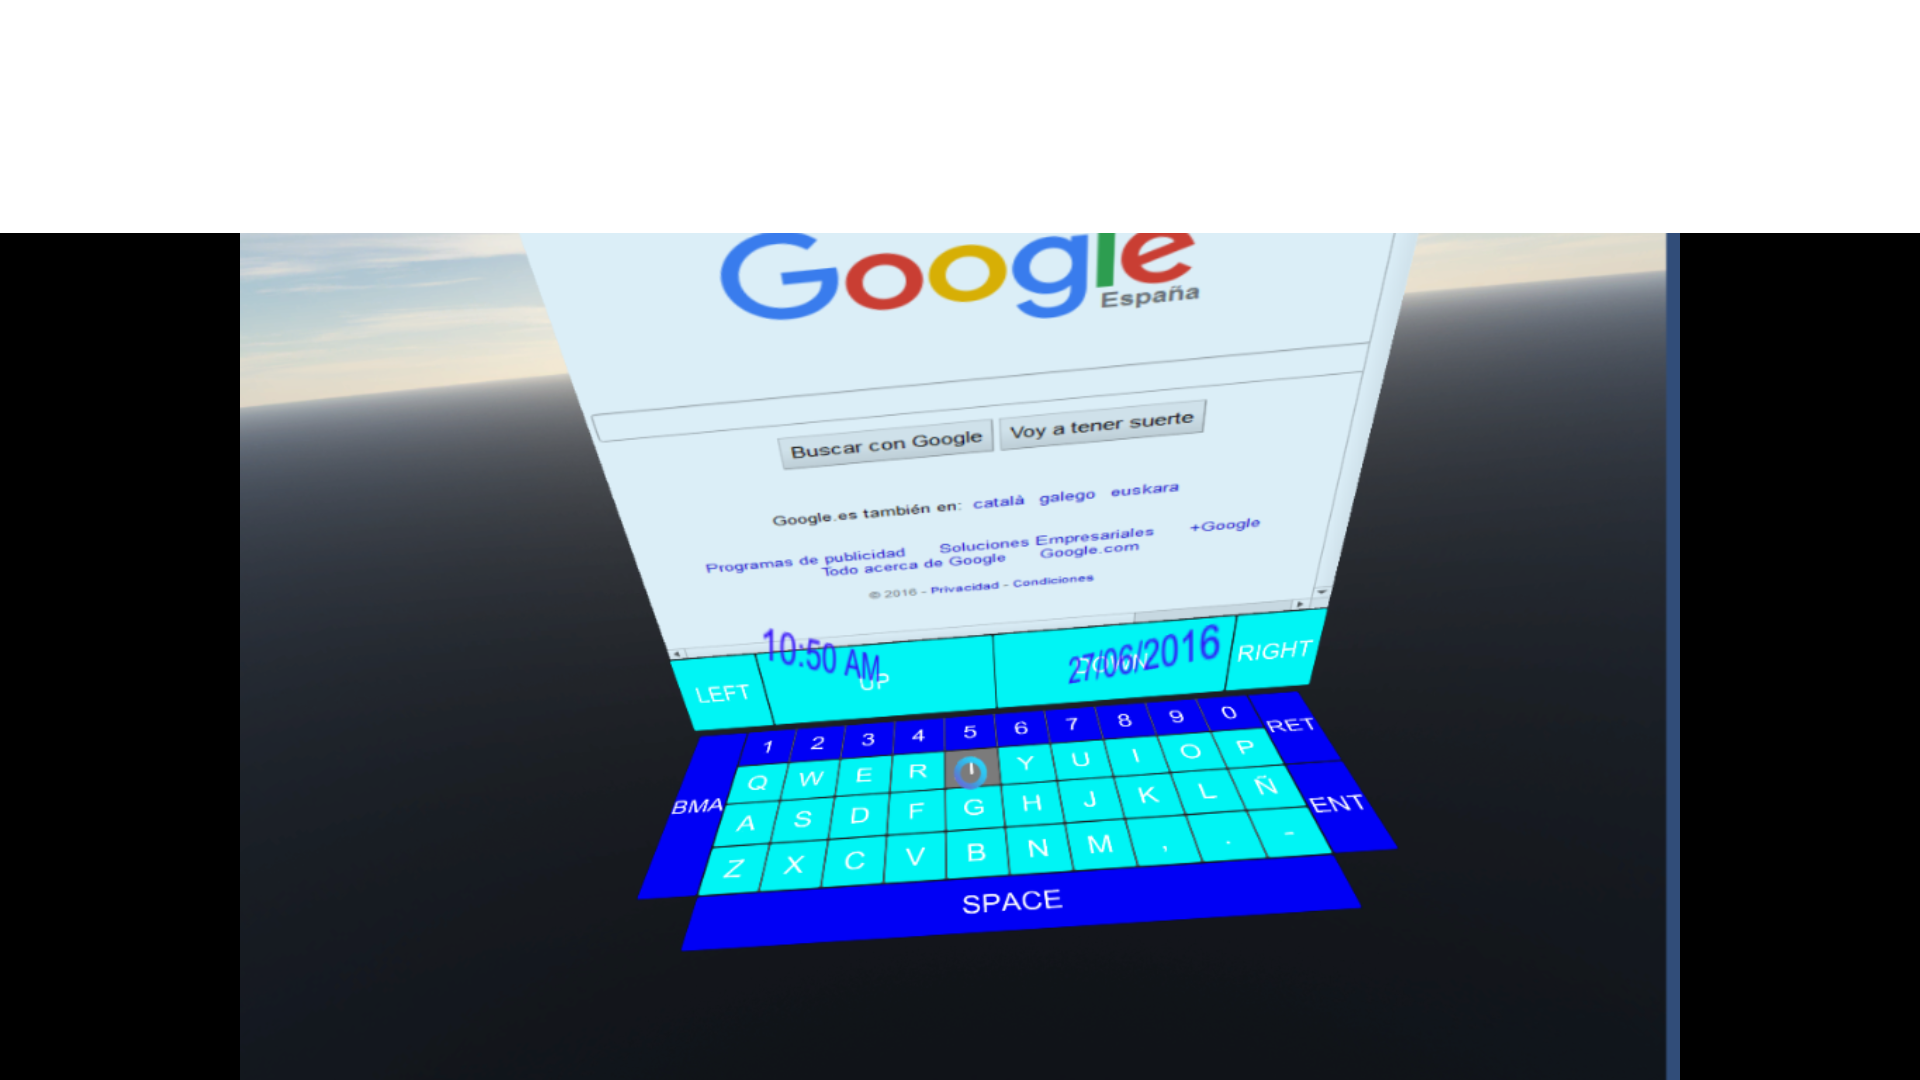
\includegraphics[width=\textwidth]{images/escritura_teclado.png} 
  \caption{Escribiendo con el teclado virtual.}
  \label{fig:writeVKB1}
\end{figure}

\begin{figure} [H]
\centering	
	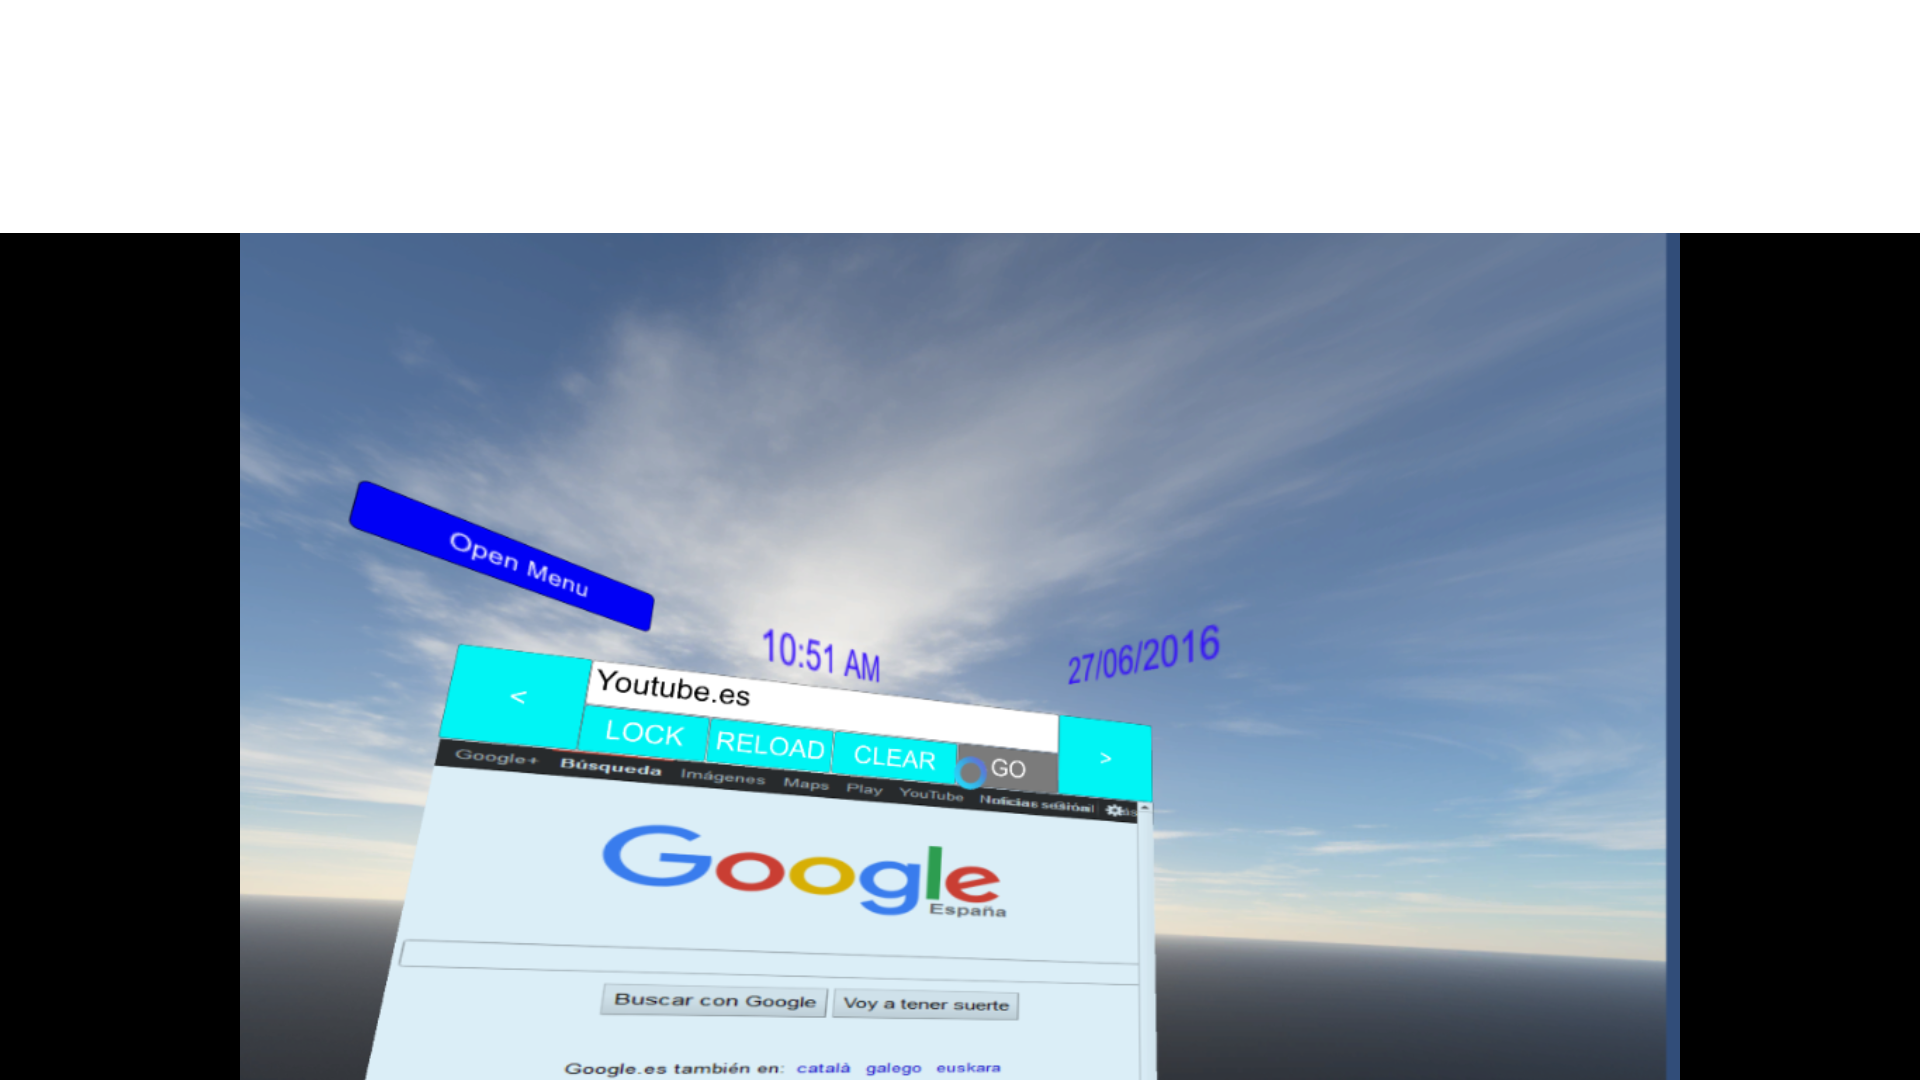
\includegraphics[width=\textwidth]{images/carga_url.png} 
  \caption{Cargando la URL.}
  \label{fig:loadURL}
\end{figure}

\begin{figure} [H]
\centering	
	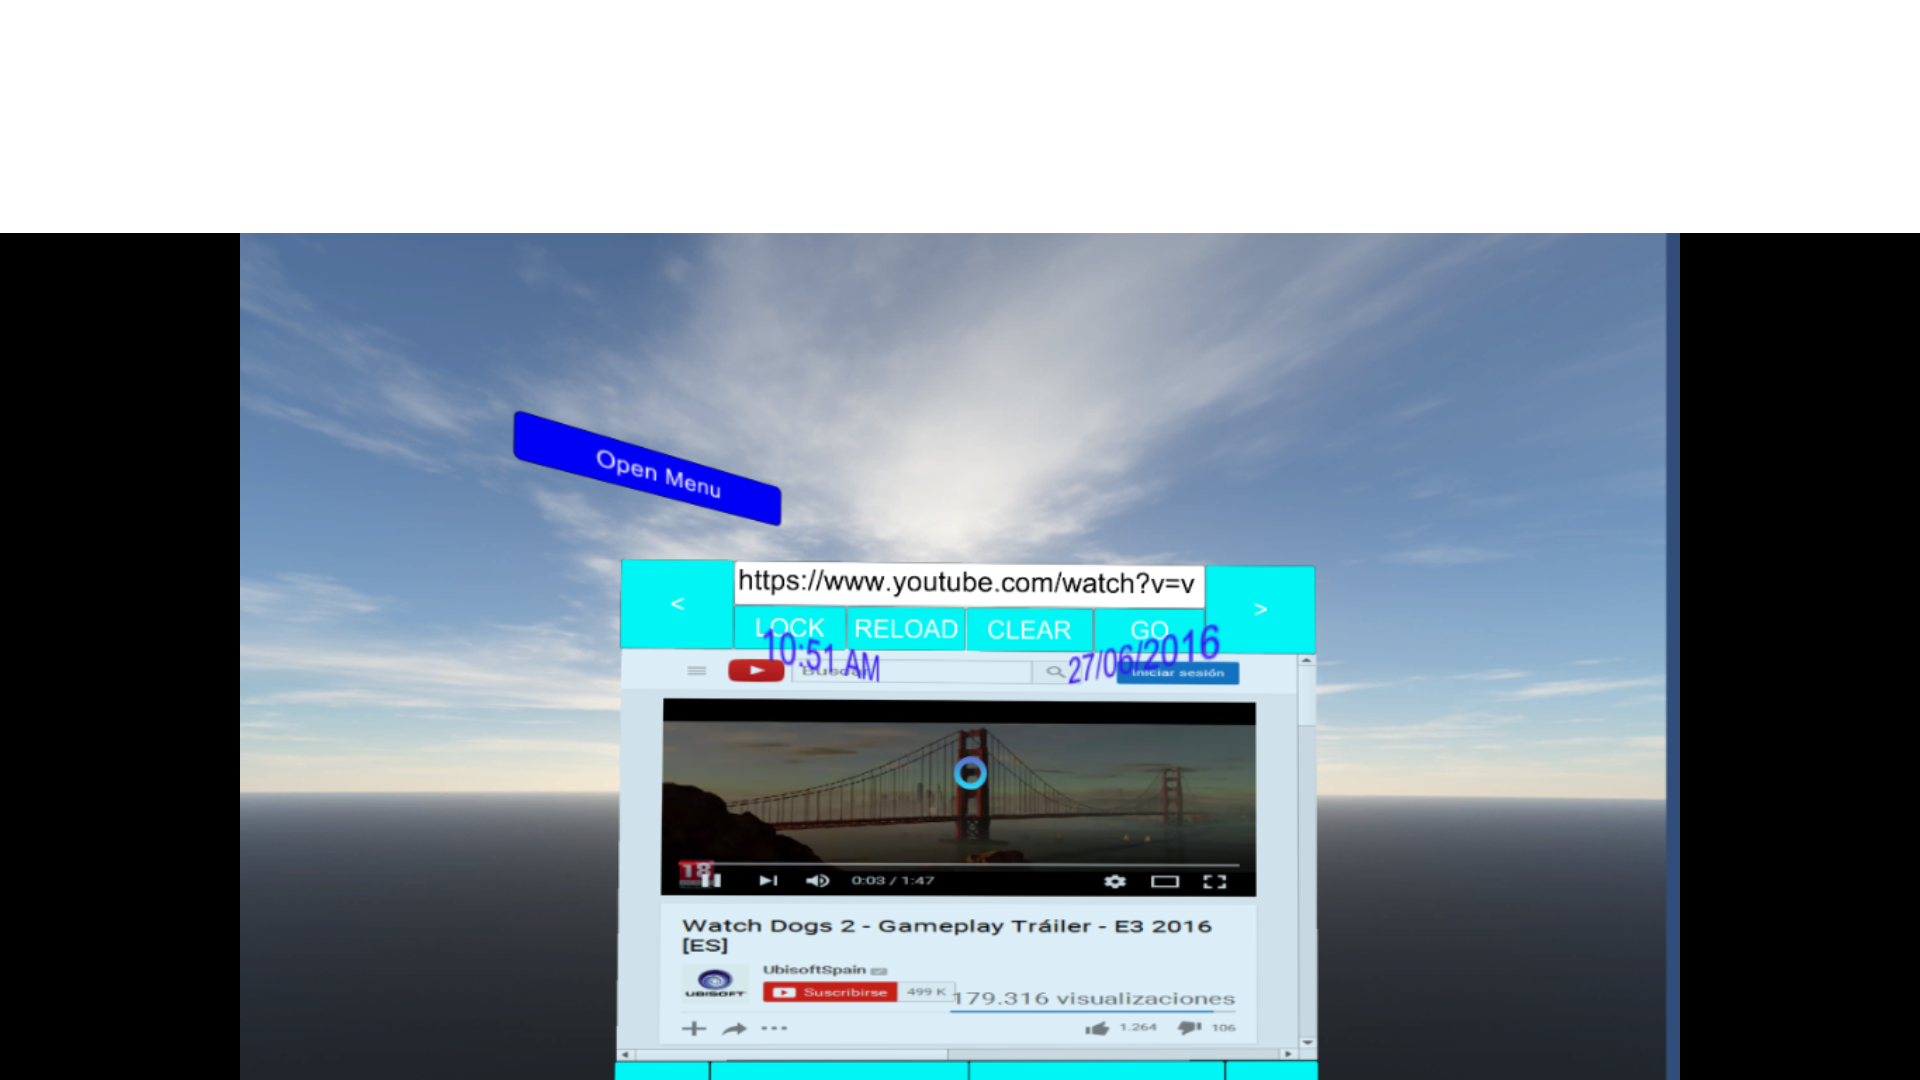
\includegraphics[width=\textwidth]{images/video.png} 
  \caption{Visualizando un v�deo.}
  \label{fig:browser2}
\end{figure}

\begin{figure} [H]
\centering	
	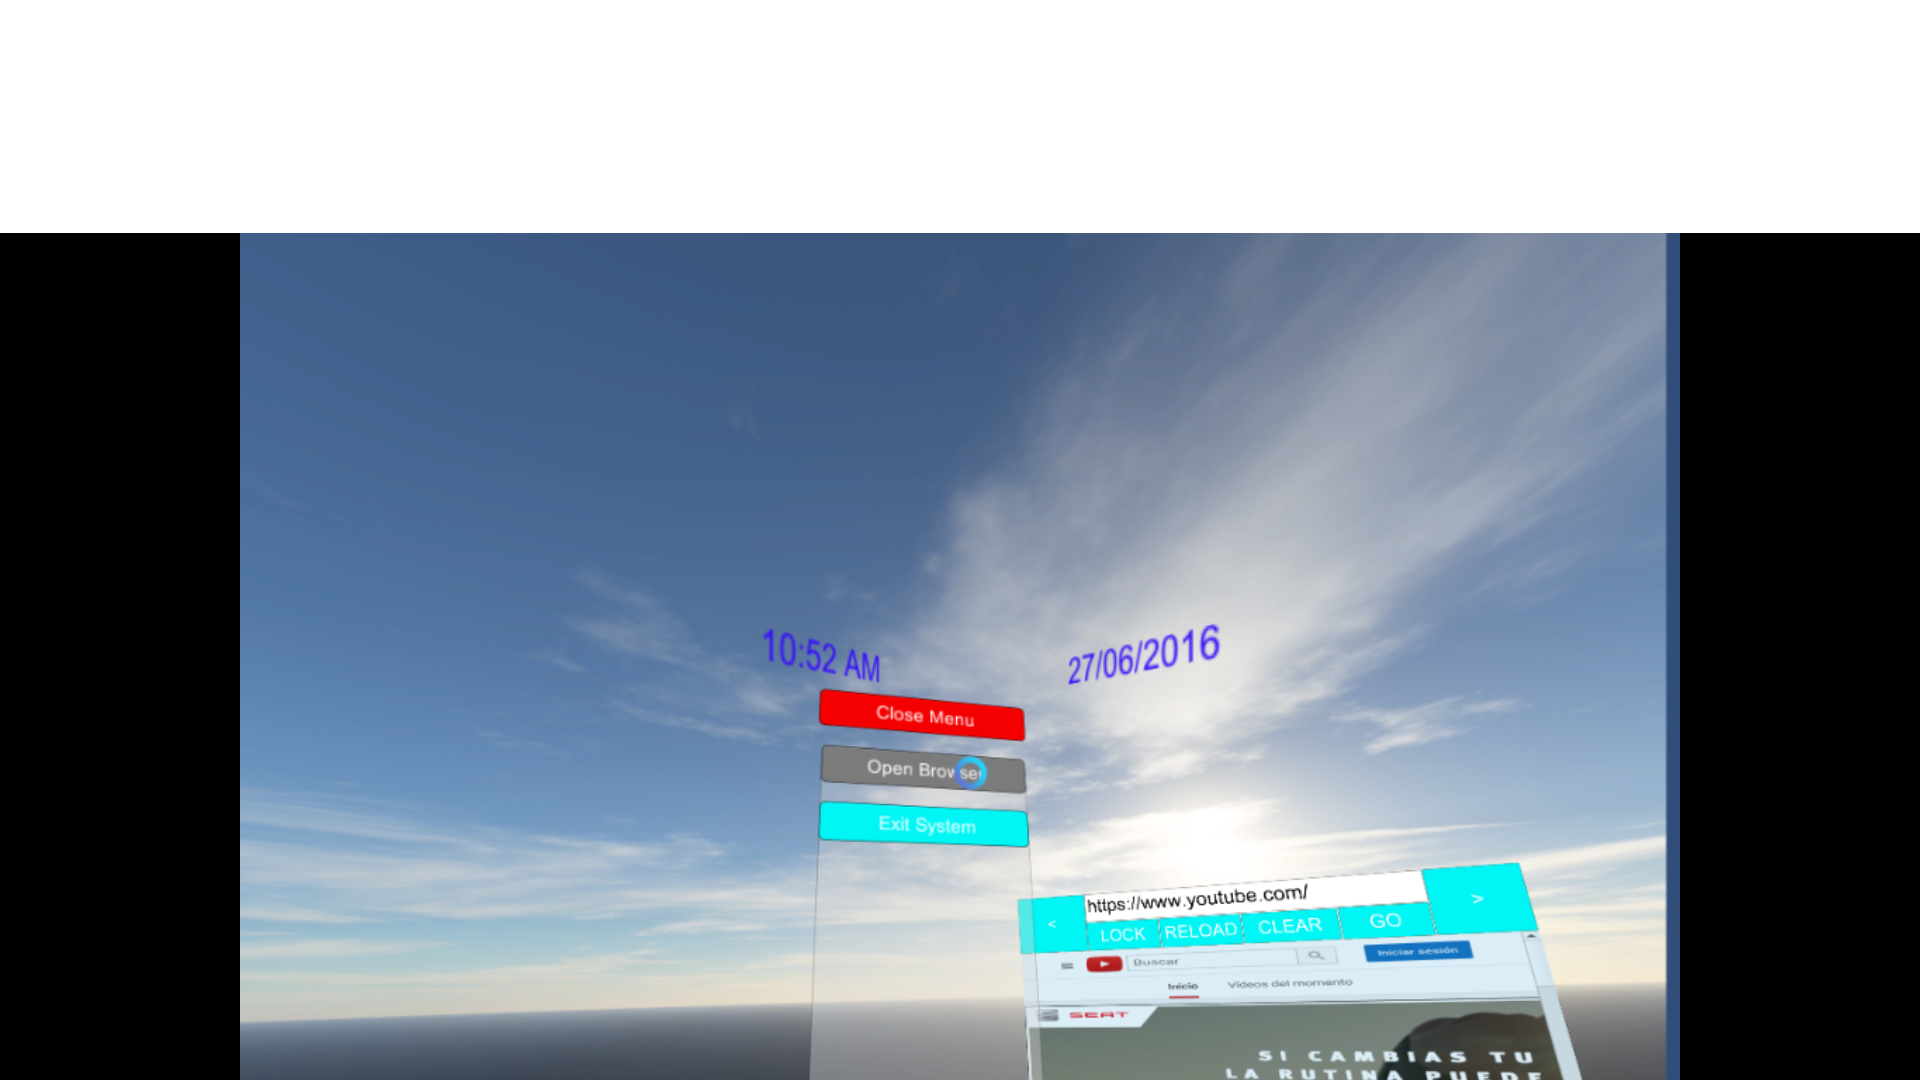
\includegraphics[width=\textwidth]{images/cierre_navegador.png} 
  \caption{Usuario seleccionado la opci�n para cerrar el navegador.}
  \label{fig:exitBrowser2}
\end{figure}

\begin{figure} [H]
\centering	
	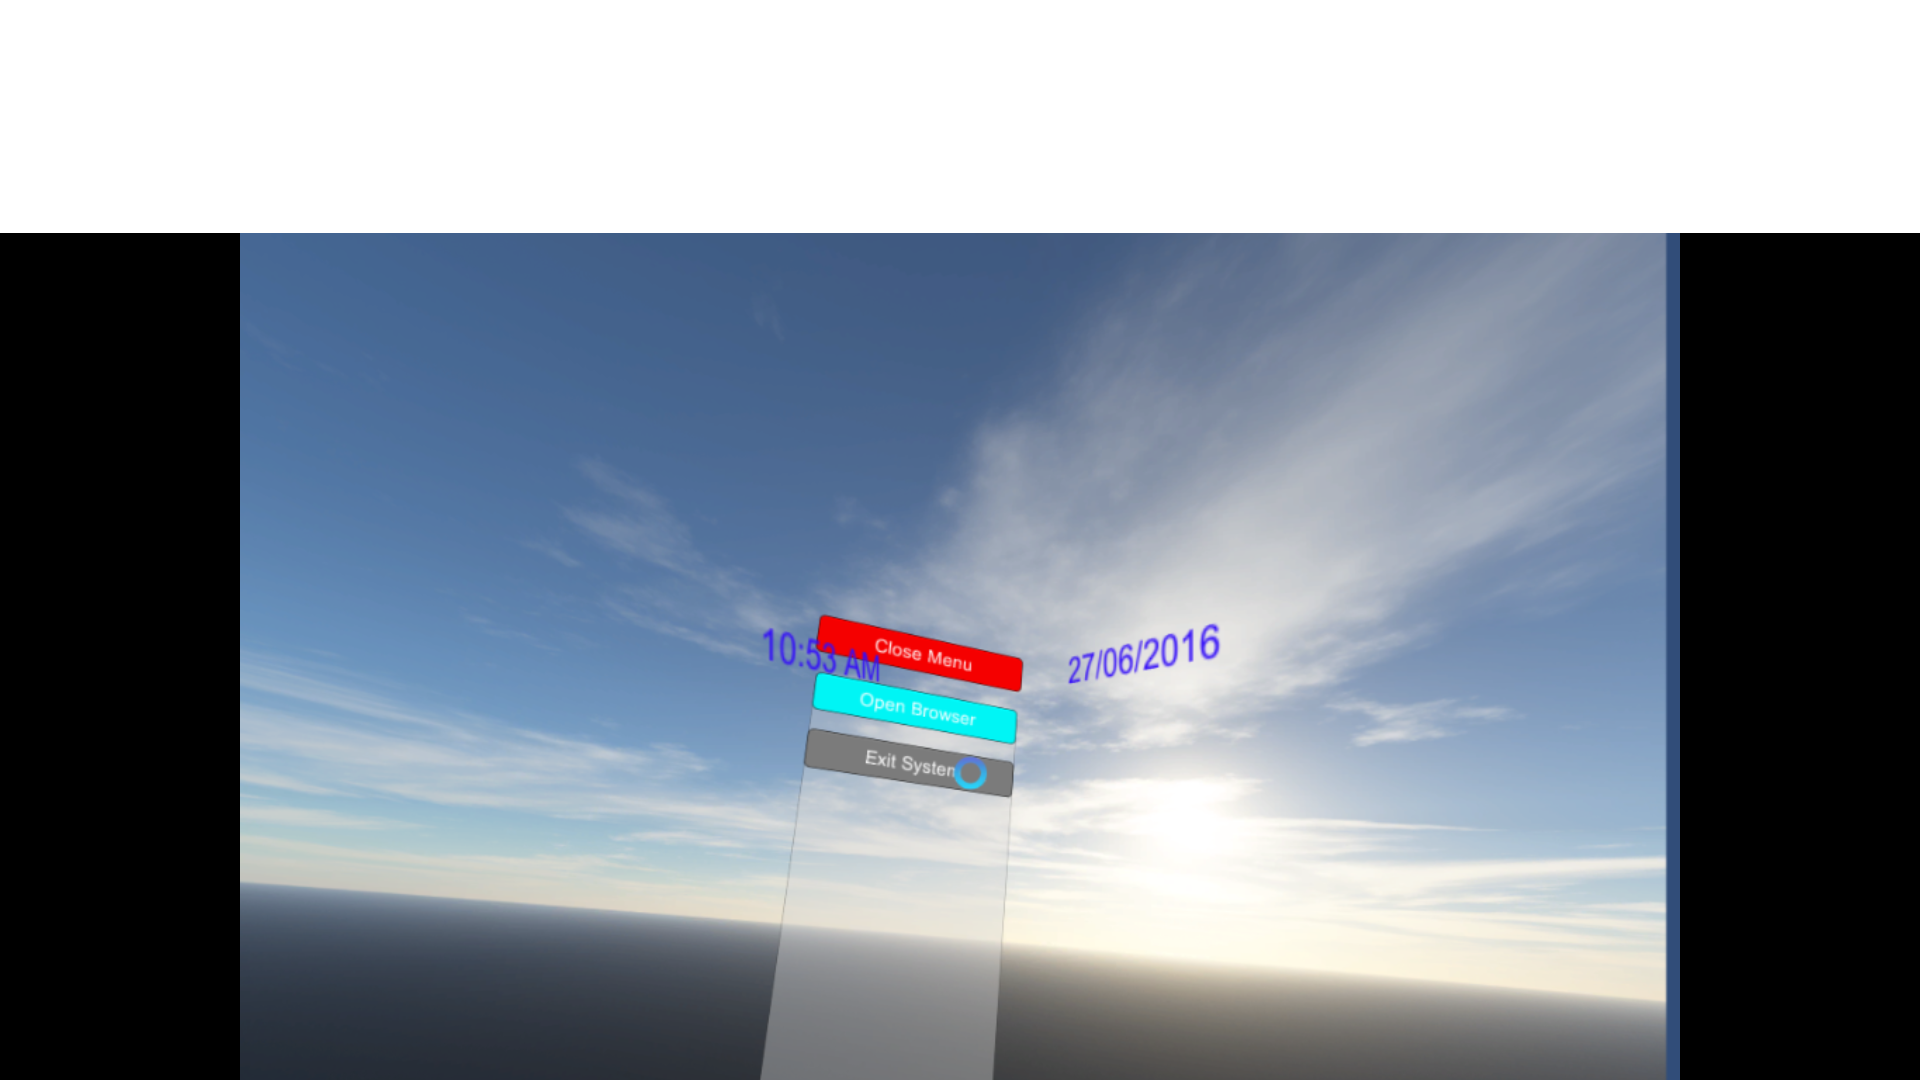
\includegraphics[width=\textwidth]{images/salir_sistema.png} 
  \caption{Usuario seleccionado la opci�n para apagar el sistema}
  \label{fig:exit3}
\end{figure}

\newpage \thispagestyle{empty} % P�gina vac�a 
